\documentclass[11pt,letterpaper]{article}
\input{headings}
\newcommand \recipeName {Moroccan Roasted Butternut Squash}
\newcommand \fileName {MoroccanRoastedButternutSquash}
\chead{\recipeName}

\begin{document}
\input{title}

I created this recipe after trying to make \href{SpicedLentilsWithPumpkin.html}{Spiced Lentils with Pumpkin} a few times. It is a Moroccan recipe by Tess Mallos that I found in {\it The food of Morocco: a journey for food lovers}. In that recipe the squash and the lentils are cooked together, with correct timing, but in a stewed fashion.  I decided to instead roast the squash with spices and add to the very end. One issue with roasting squash is that often it falls apart into a mush. Thus I remembered that my Mom, Dioraci Urtassum, makes a sweet squash dish where it is cooked for a long time in sirup and never falls apart. The secret it to use calcium to set the pectin in the squash before cooking it. Thus I resorted to pickle crisp, which is a calcium product used to ensure that pickles remain crisp. In Edmonton I found pickle crisp at Canadian Tire.

\begin{description}

\item[Ingredients:]\ \\
	\begin{itemize}
	\item 1 1/2 tablespoon of pickle crisp
	\item 1 small butternut squash (1 1/2 to 2 pounds)
	\item 1/2 teaspoon of salt
	\item 1 teaspoon of turmeric
	\item 1/2 teaspoon of paprika
	\item 1/2 teaspoon of cumin
	\item 2 tablespoon of olive oil
	\end{itemize}

\item[Procedure:]\ \\
	\begin{enumerate}
	\item {\bf Prepare the pumping}
	\begin{itemize}
	\item Peel the pumpkin removing all the white part of the peel.
	\item Cut the pumpkin in 3/4-inch cubes.
	\item Mix one tablespoon of pickle crisp with half gallon of cold water.
	\item Put the pumpkin in the water and let soak for at least 45 minutes. It can soak overnight.
	\end{itemize}
	\item {\bf Season the pumpkin}
	\begin{itemize}
	\item Drain the pumpkin and rinse under running cold water.
	\item Leave in a colander or strainer until most of the water has dripped off.
	\item Mix the spices in a small bowl.
	\item Sprinkle the salt over the pumpkin tossing by lifting the bowl.
	\item Sprinkle the spices on the salted pumpkin.
	\item Let it seat for at least 45 minutes, but up to several hours.
	\end{itemize}
	\item {\bf Roast the pumpkin}
	\begin{itemize}
	\item Put a light colour metal rimmed baking sheet in the over.
	\item Pre-heat the oven to 350 F.
	\item Once the oven is hot, remove the hot baking sheet from the oven, and put the olive oil on it making sure to spread over a large area in the center
	\item Transfer the seasoned pumpkin from the bowl onto the oiled baking sheet and put back in the oven.
	\item Roast for 45 minutes.
	\item Using a spatula, turn the pumpkin pieces around, rotate the baking sheet.
	\item Continue roasting for another 15 to 30 minutes until a sharp paring knife pierces through the pieces of pumpkin easily
	\end{itemize}
	\item {\bf Serving or using in another recipe}
	\begin{itemize}
	\item You can serve warm immediately after roasting.
	\item If using in another recipe, it can be prepared a day in advance, cooled, placed into the refrigerator, and warmed up either in the over or in the microwave the next day.
	\end{itemize}
	\end{enumerate}
\end{description}

\begin{table}
\begin{tabular}{cccc}
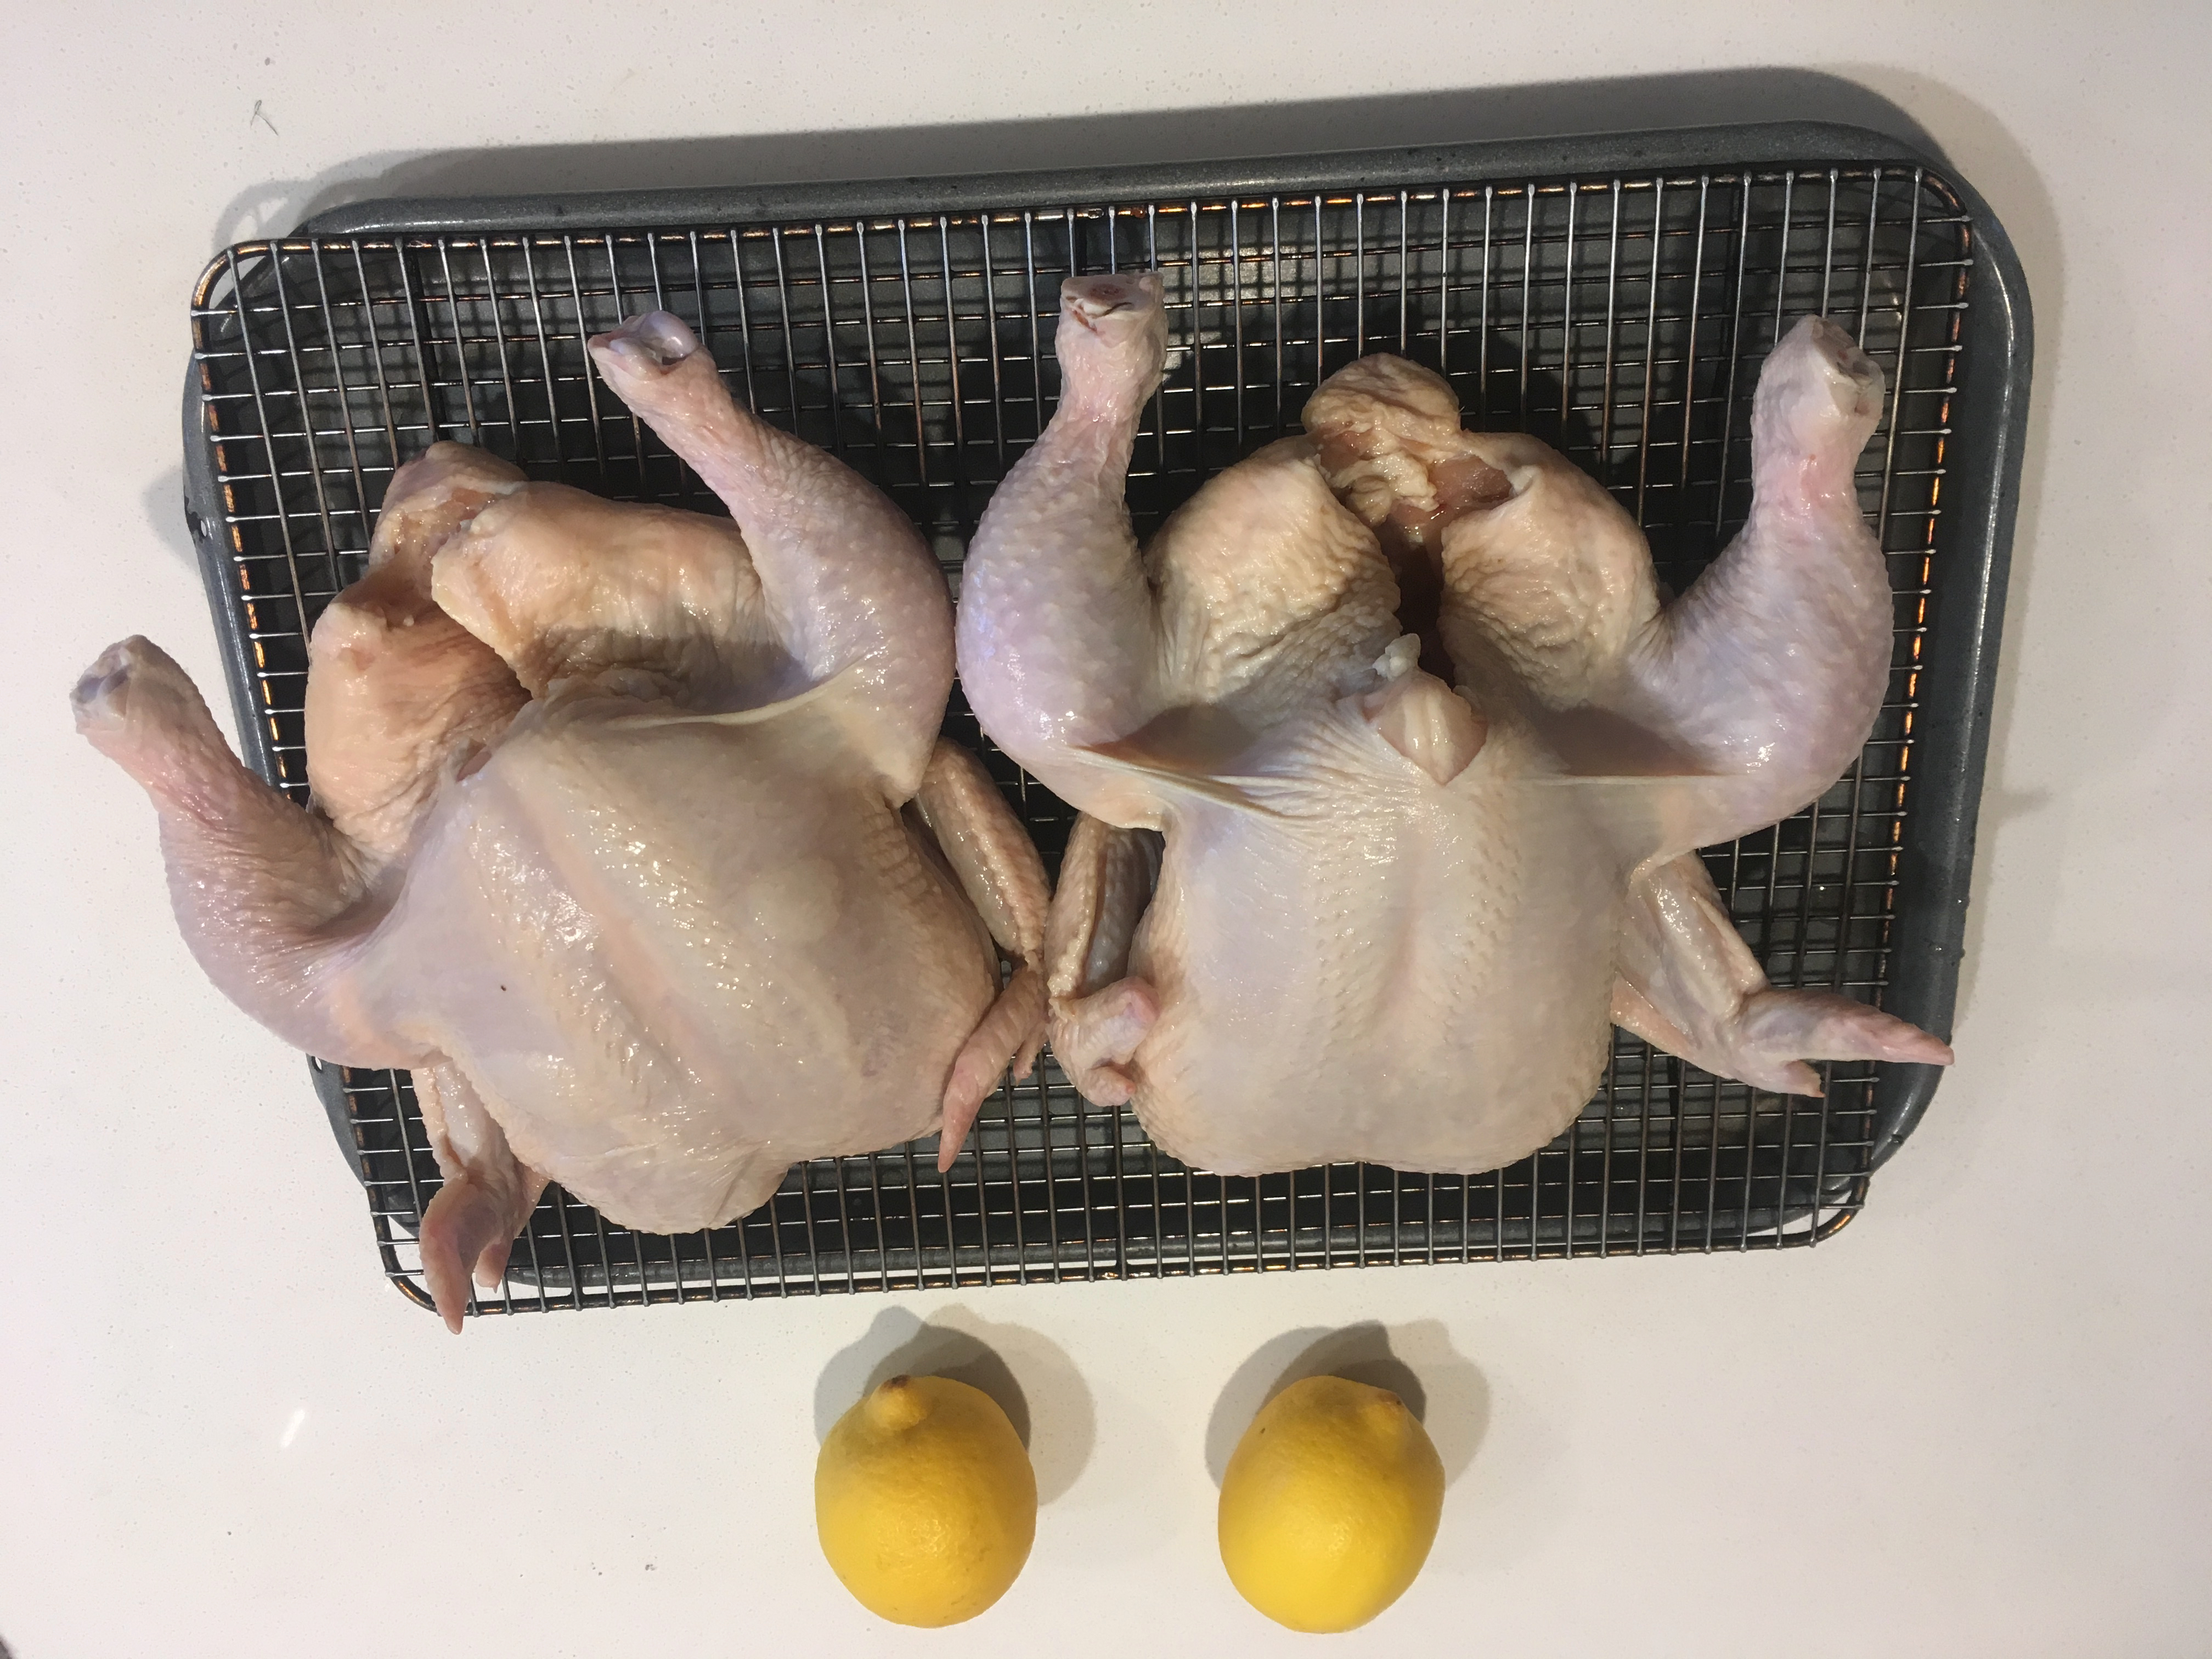
\includegraphics[width=0.25\textwidth]{\imageDir/\fileName/IMG_3197.jpg} &
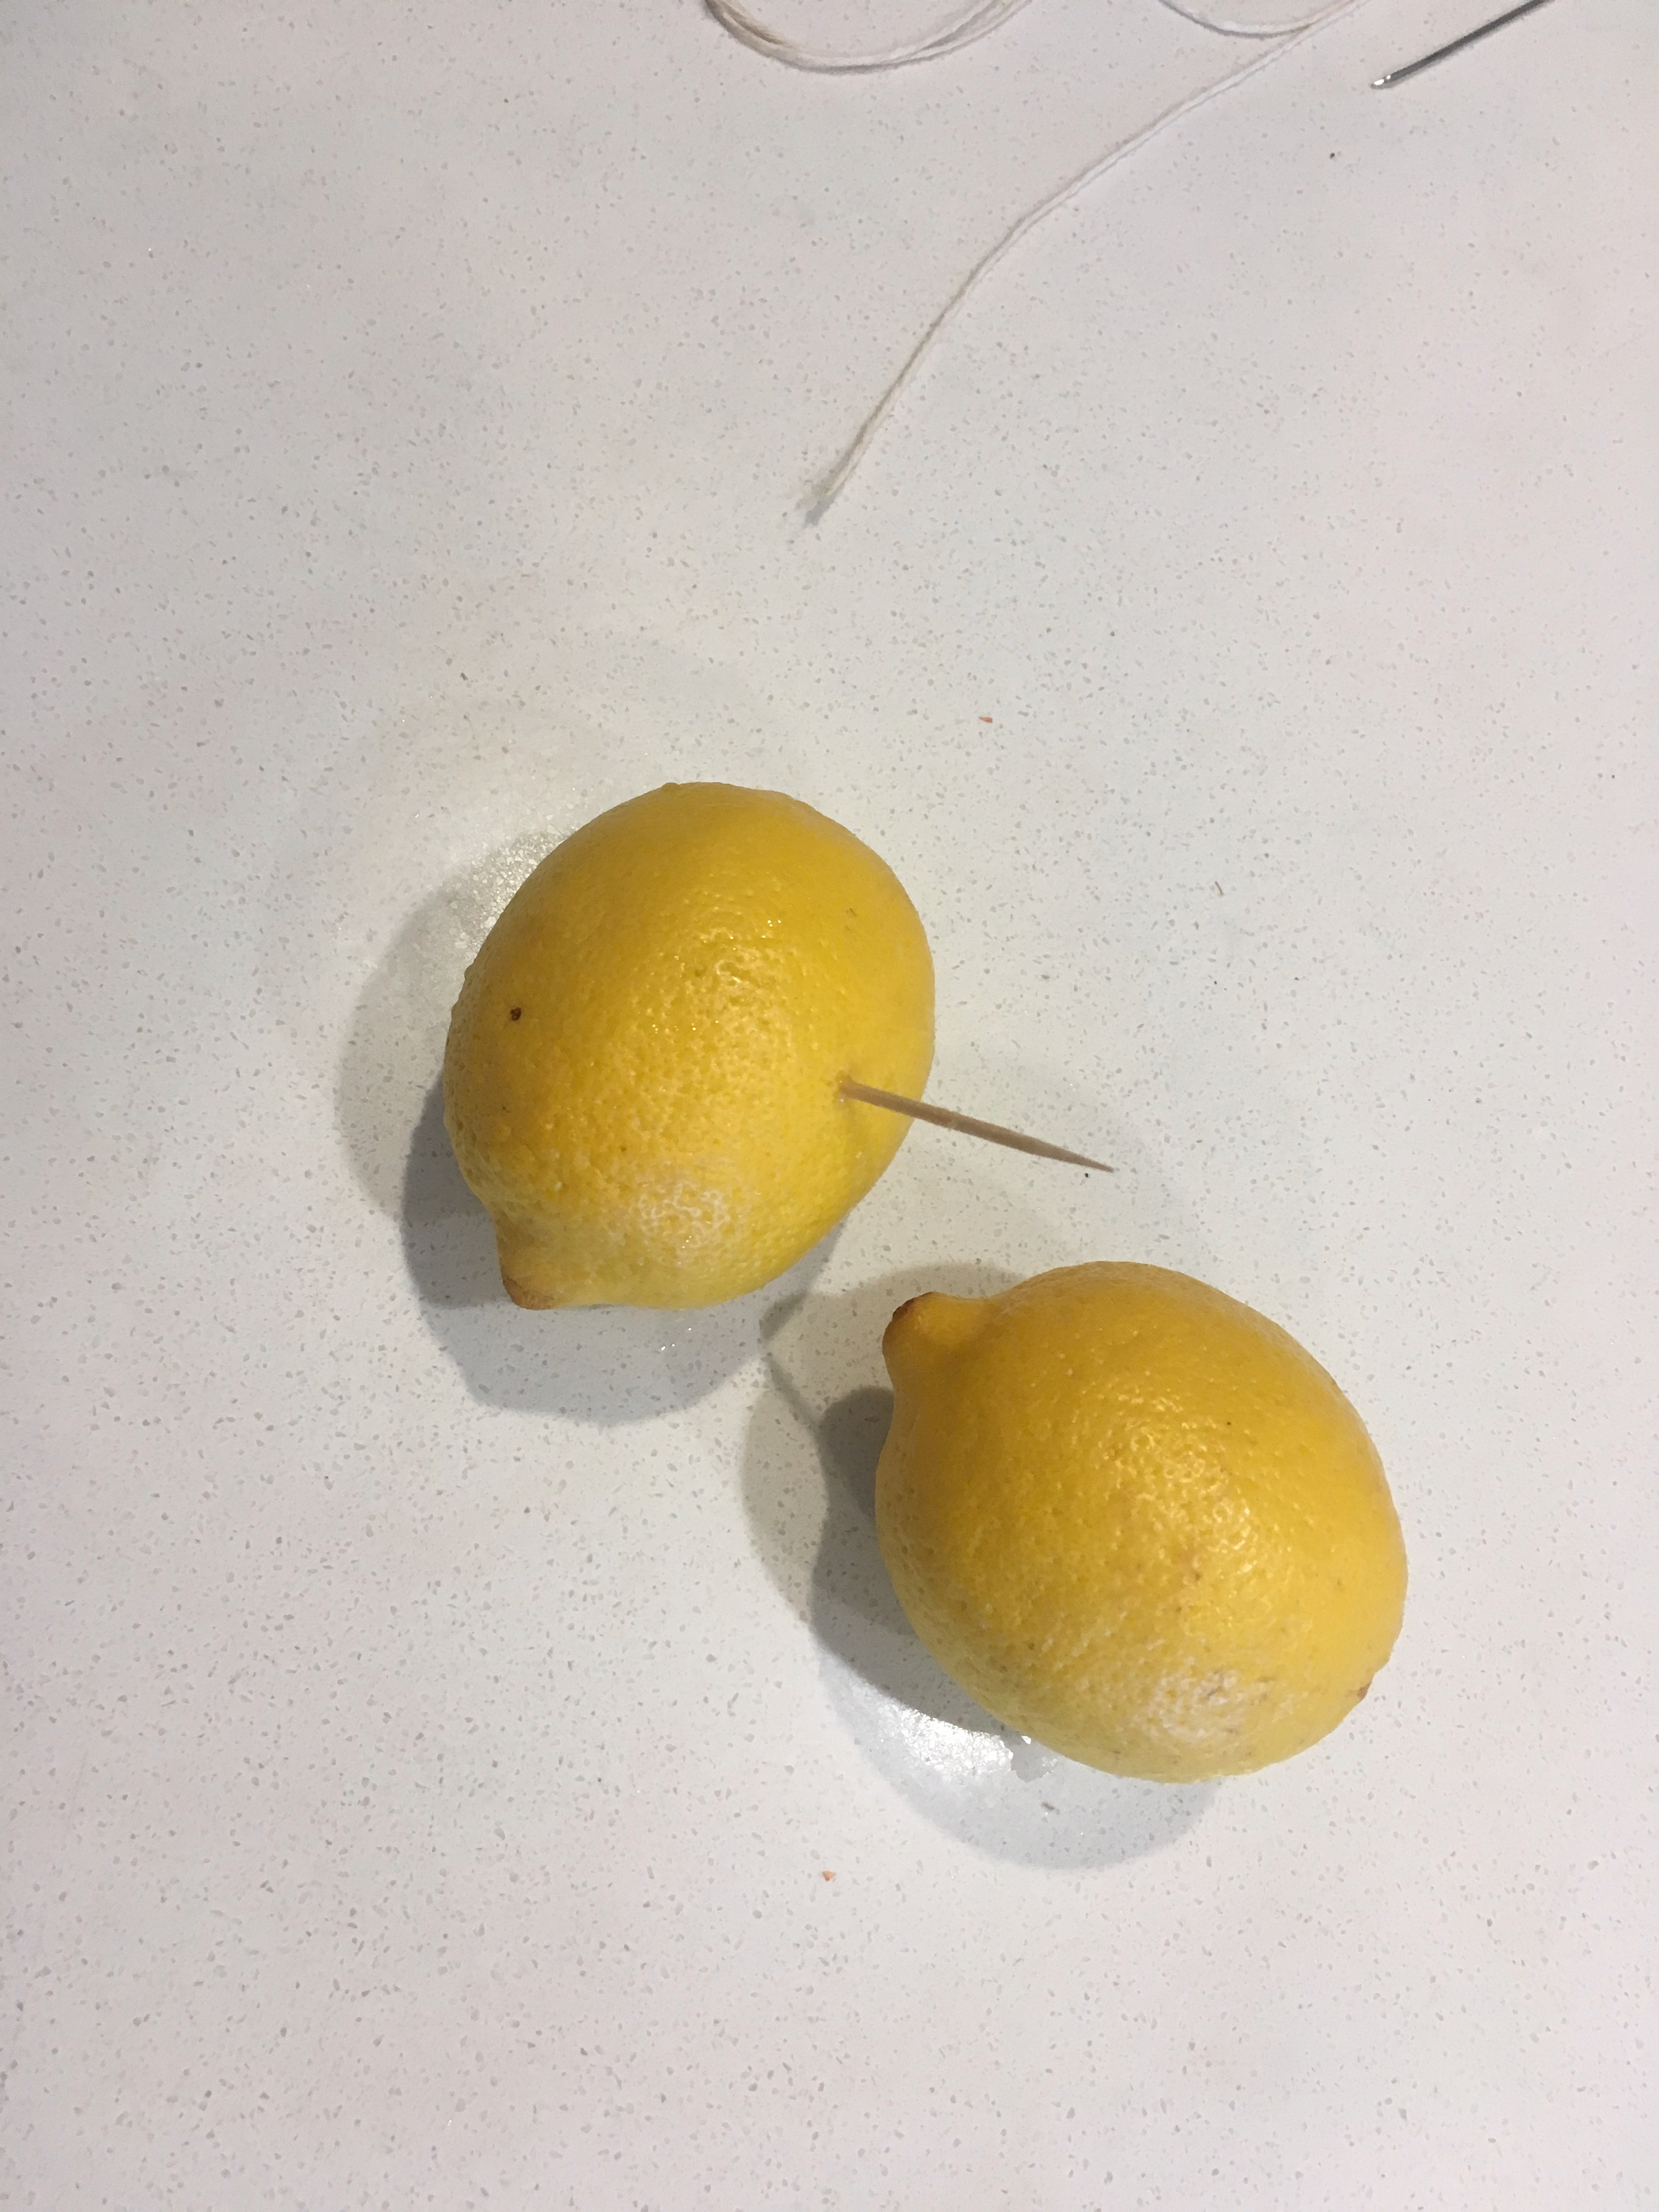
\includegraphics[width=0.25\textwidth]{\imageDir/\fileName/IMG_3212.jpg} &
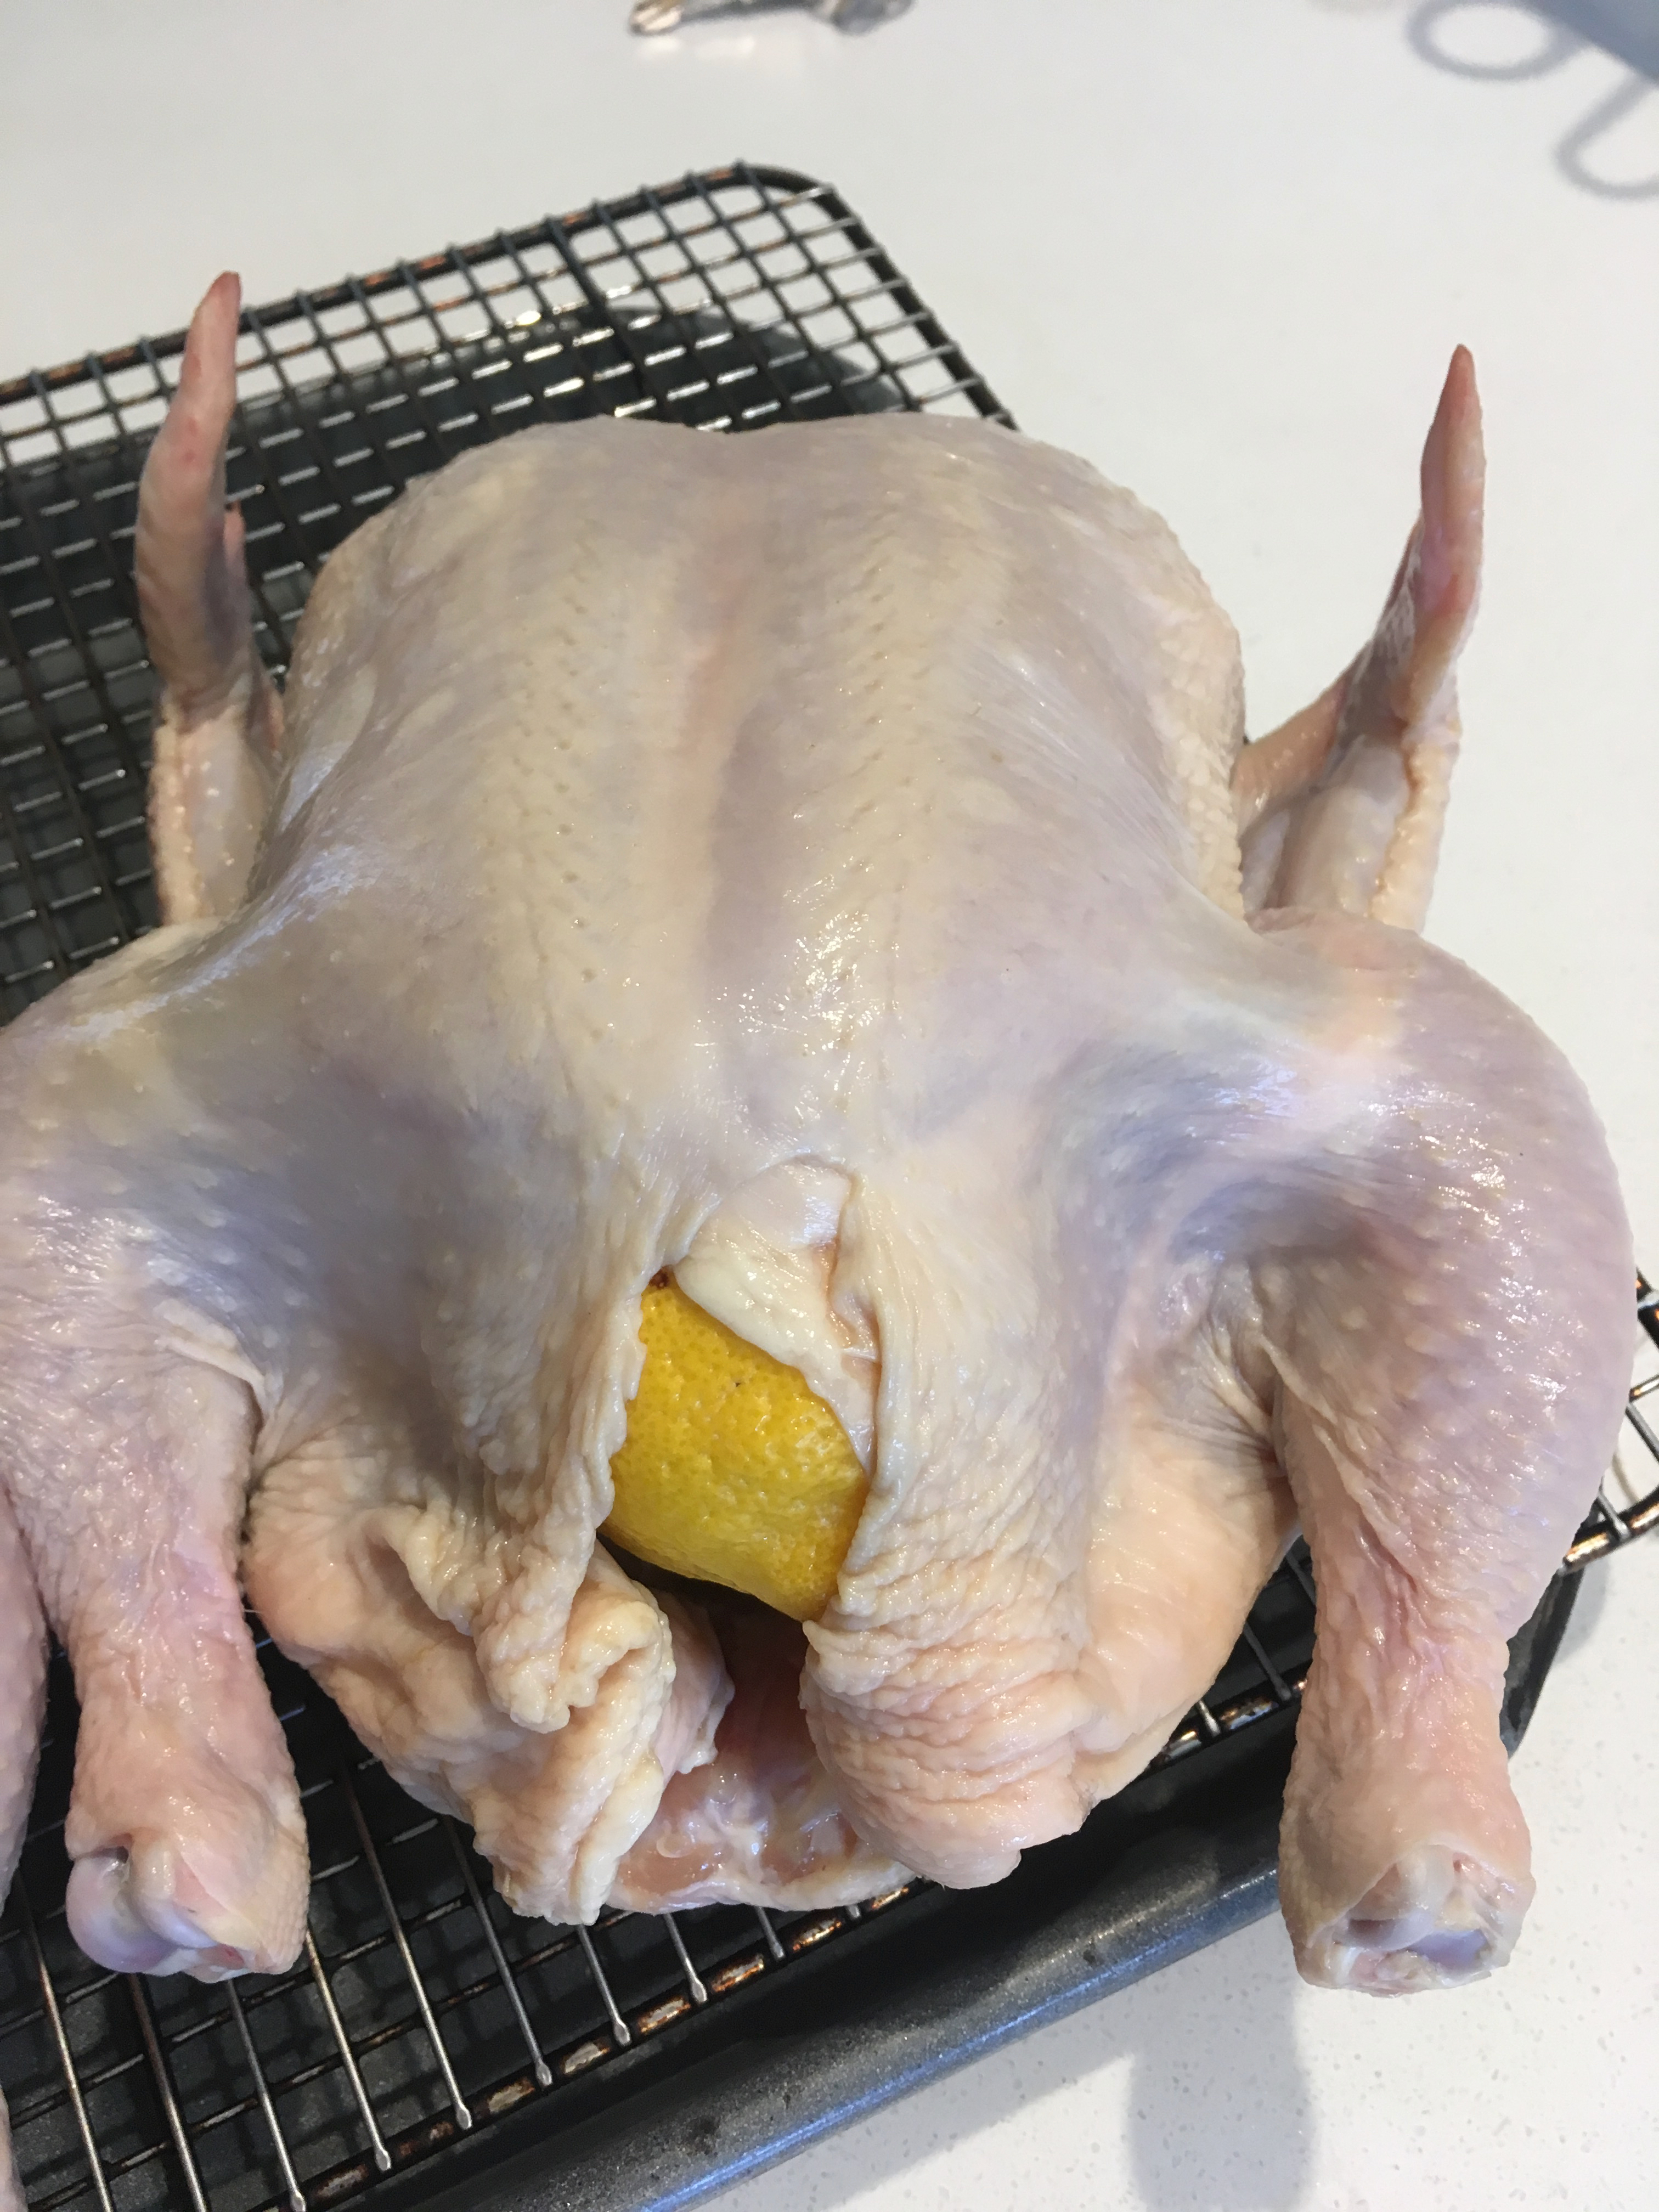
\includegraphics[width=0.25\textwidth]{\imageDir/\fileName/IMG_3213.jpg} \\
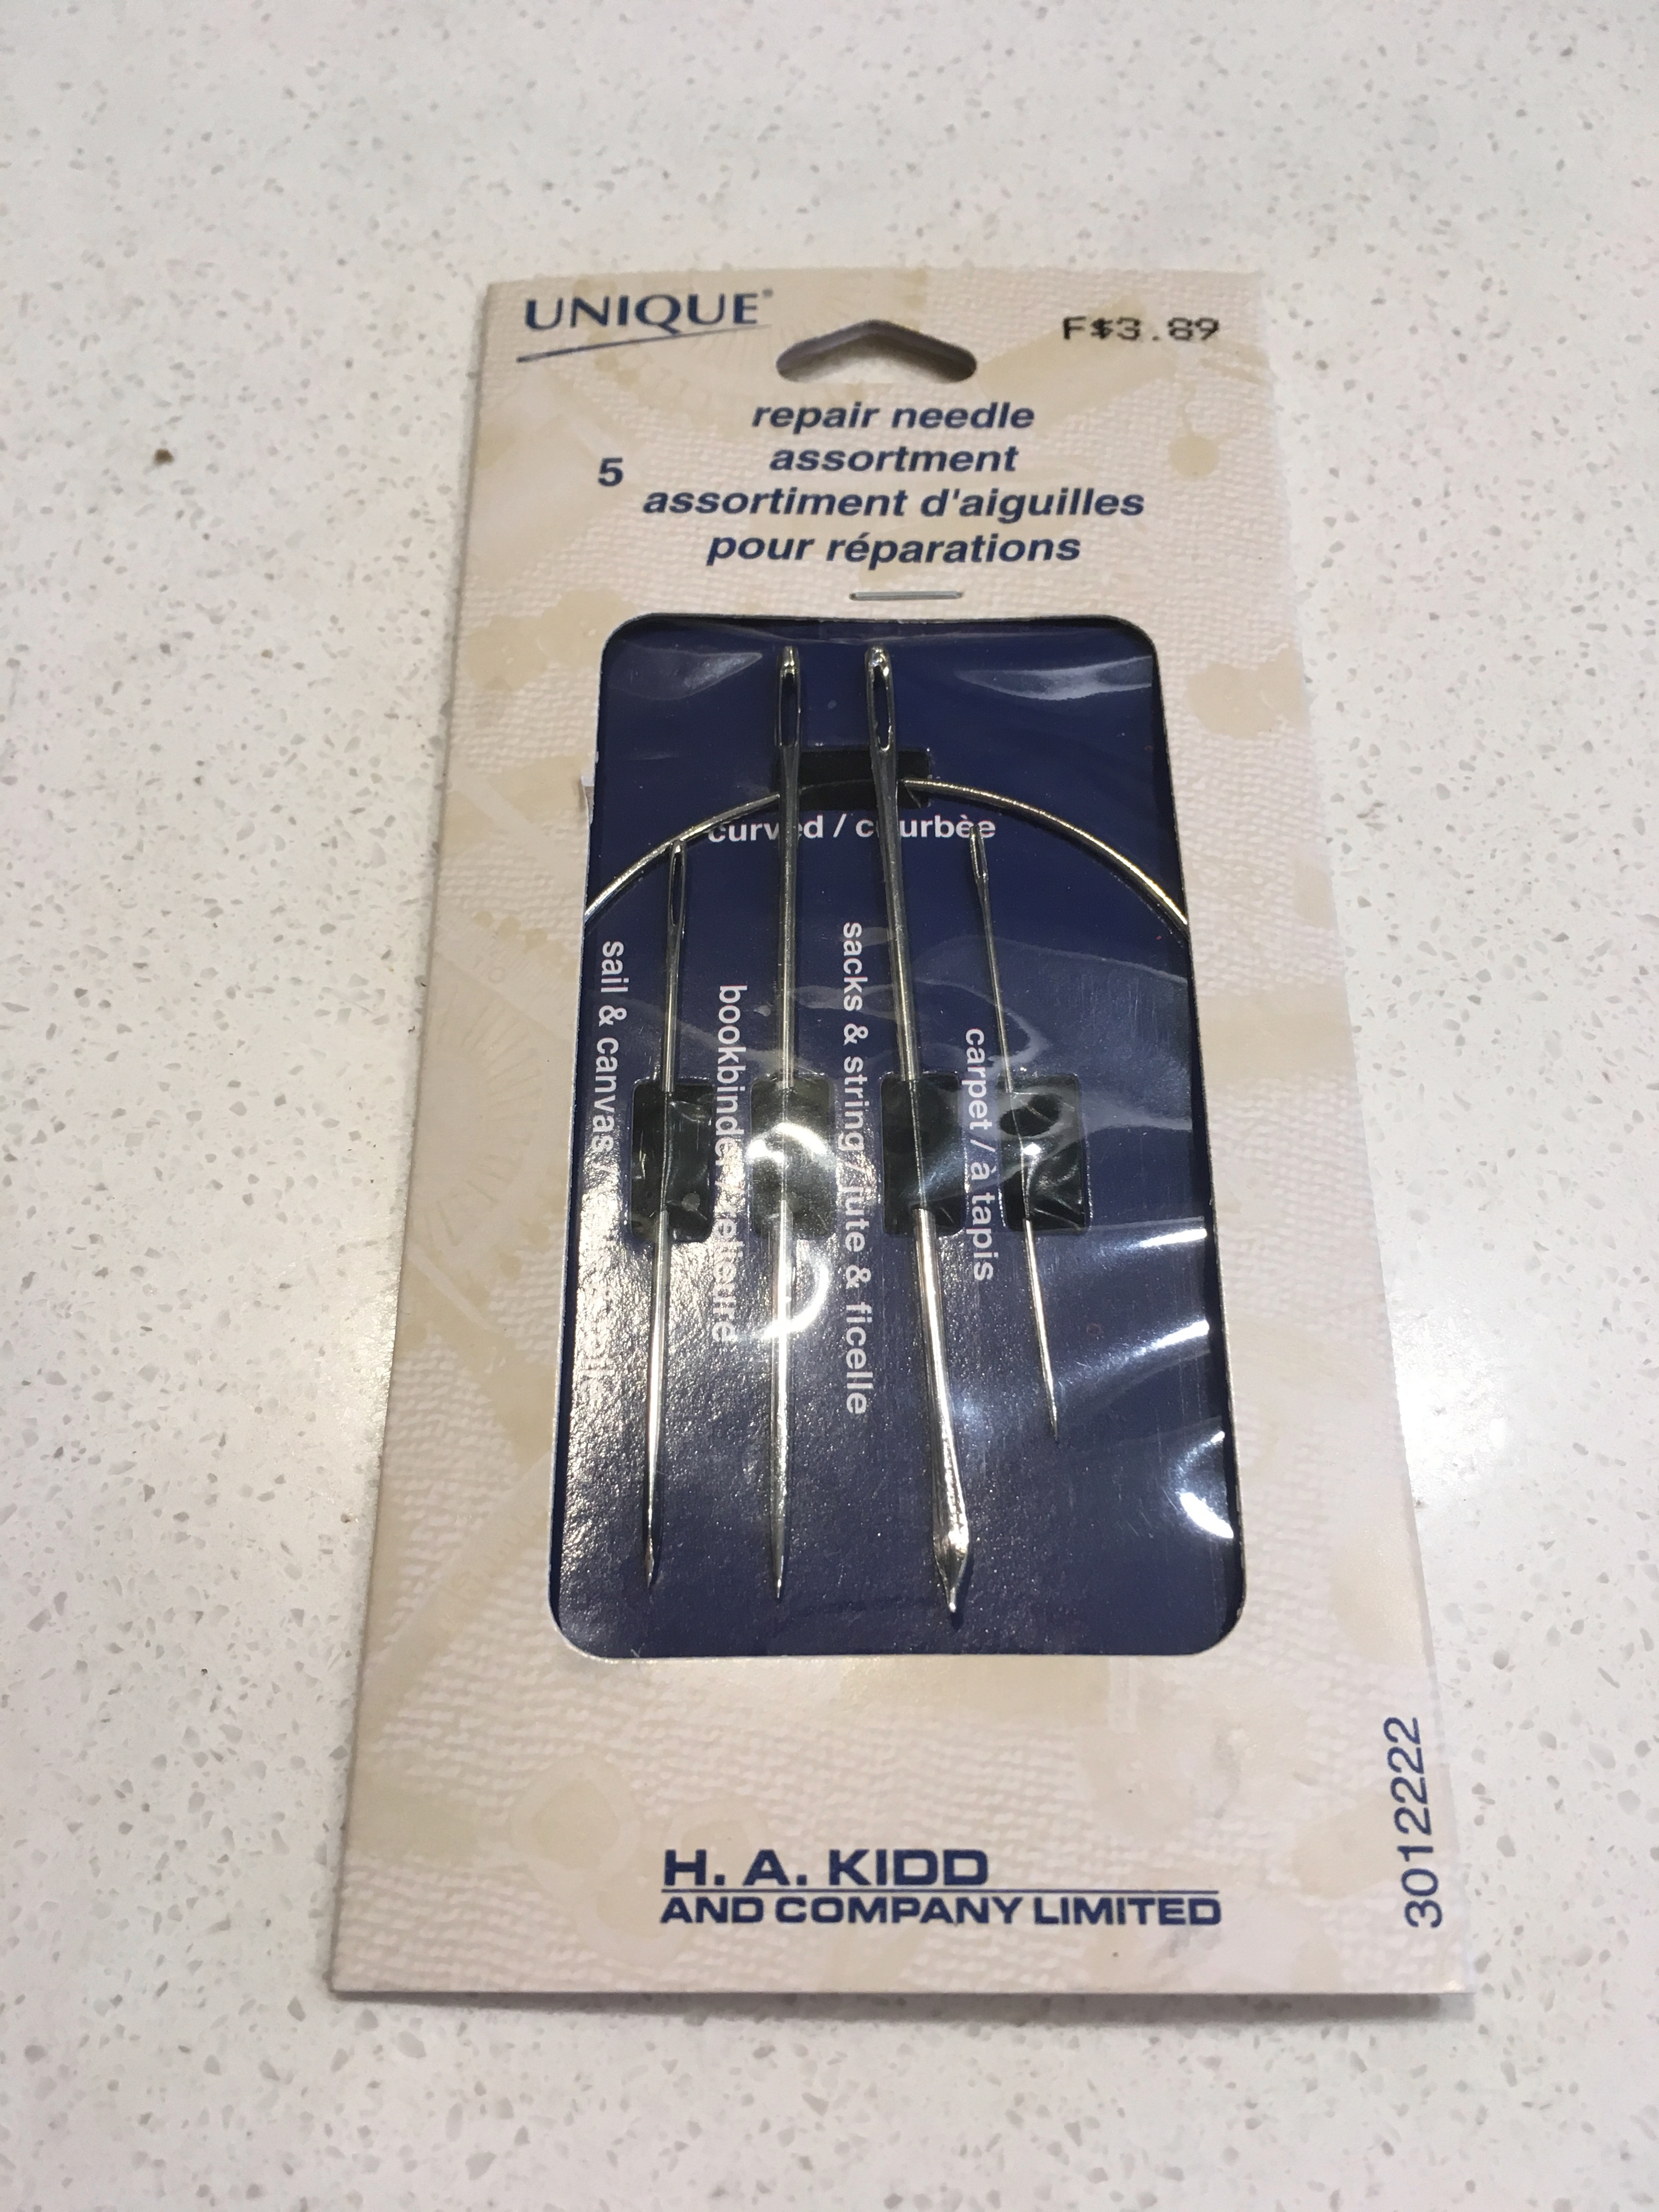
\includegraphics[width=0.25\textwidth]{\imageDir/\fileName/IMG_3206.jpg} &
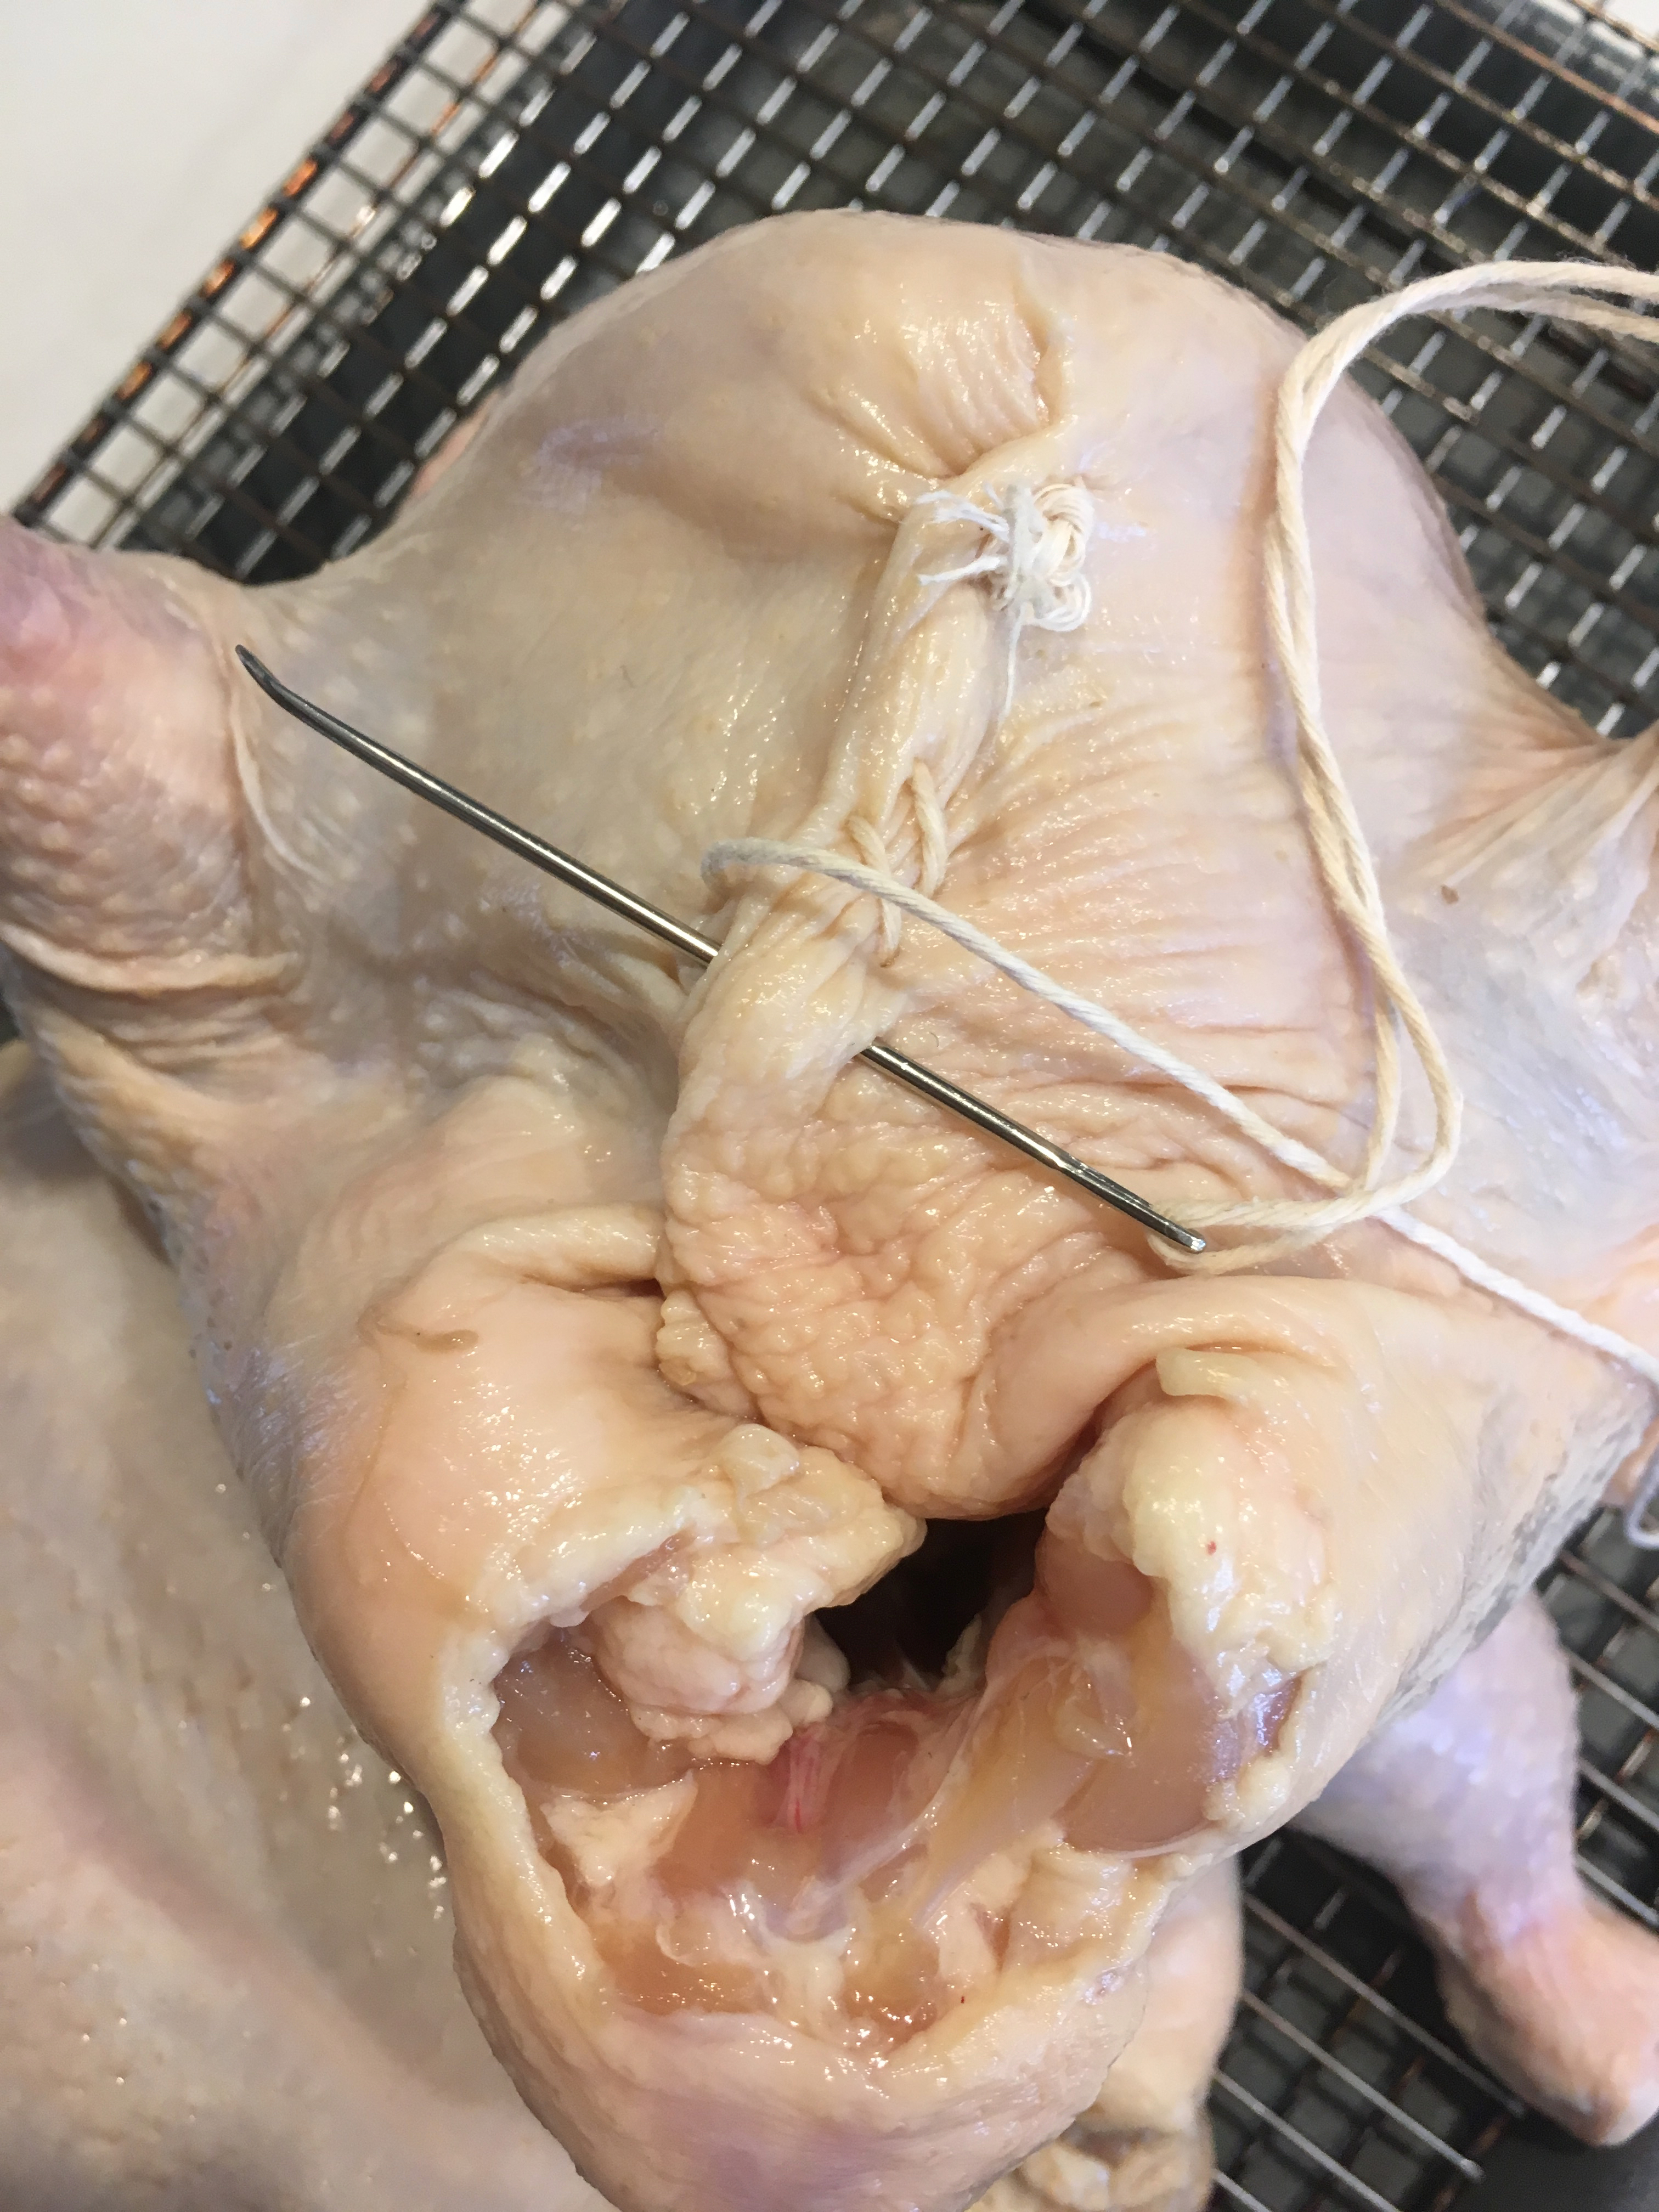
\includegraphics[width=0.25\textwidth]{\imageDir/\fileName/IMG_3214.jpg} &
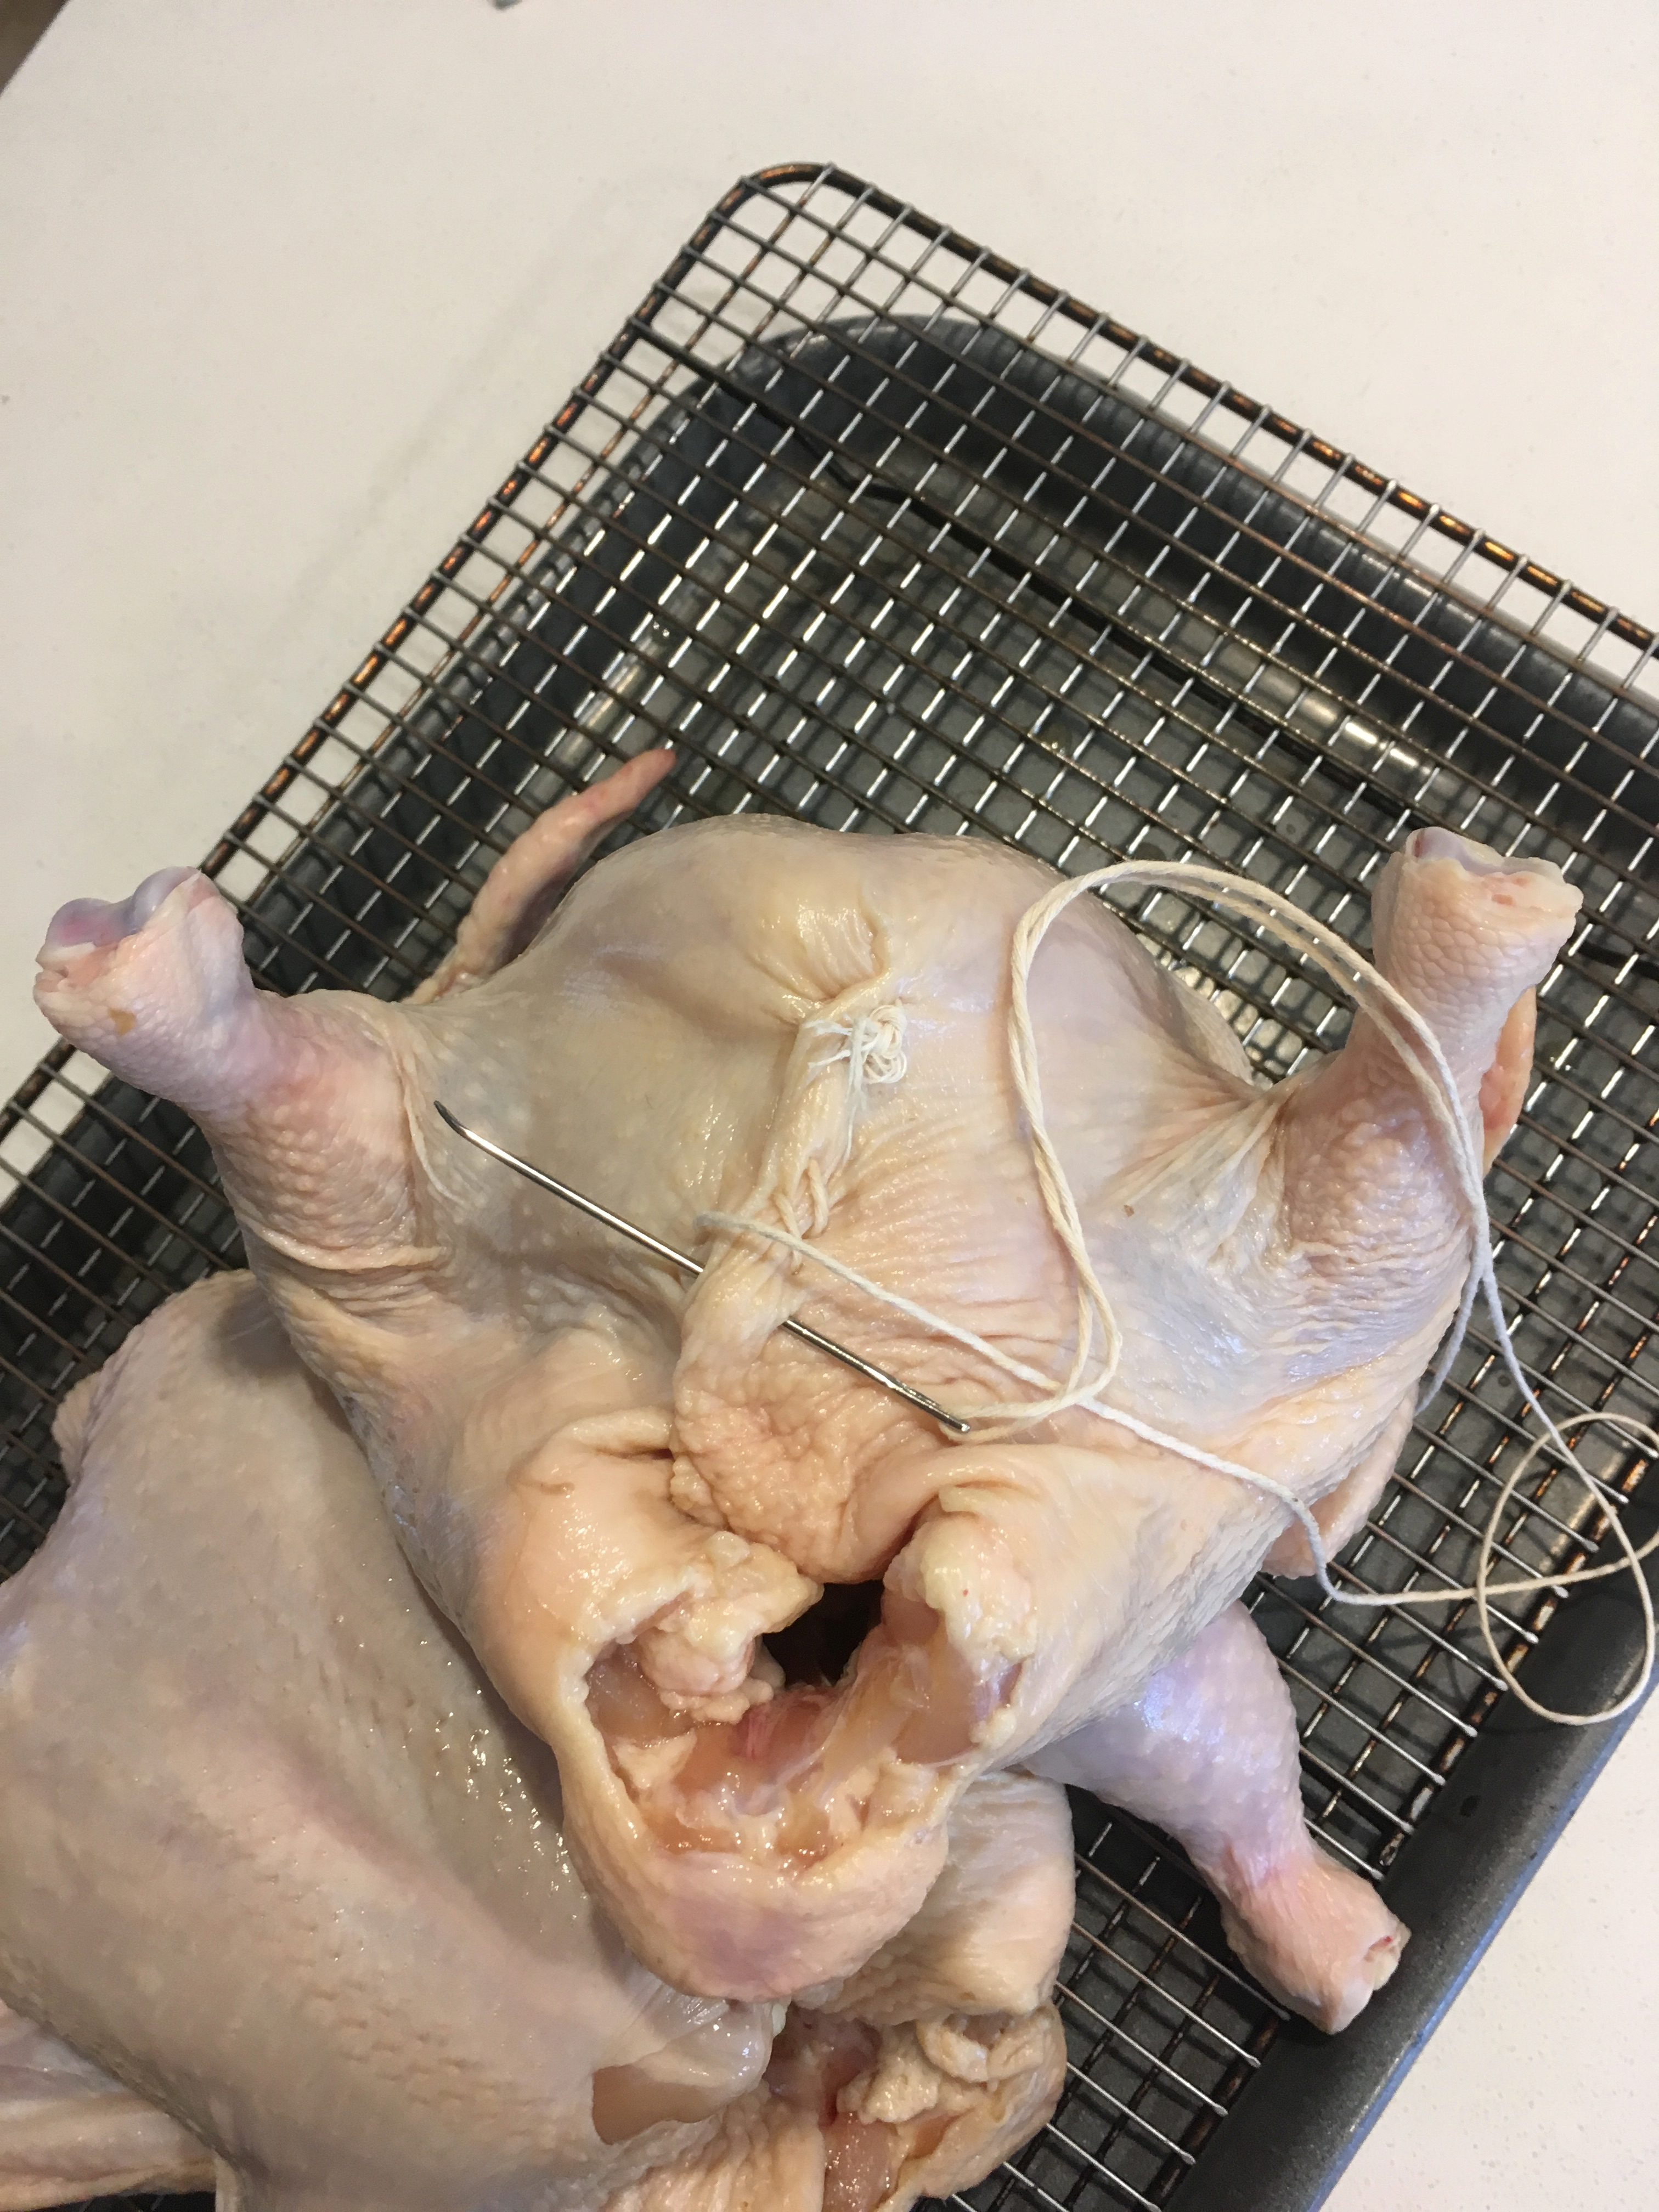
\includegraphics[width=0.25\textwidth]{\imageDir/\fileName/IMG_3216.jpg} \\
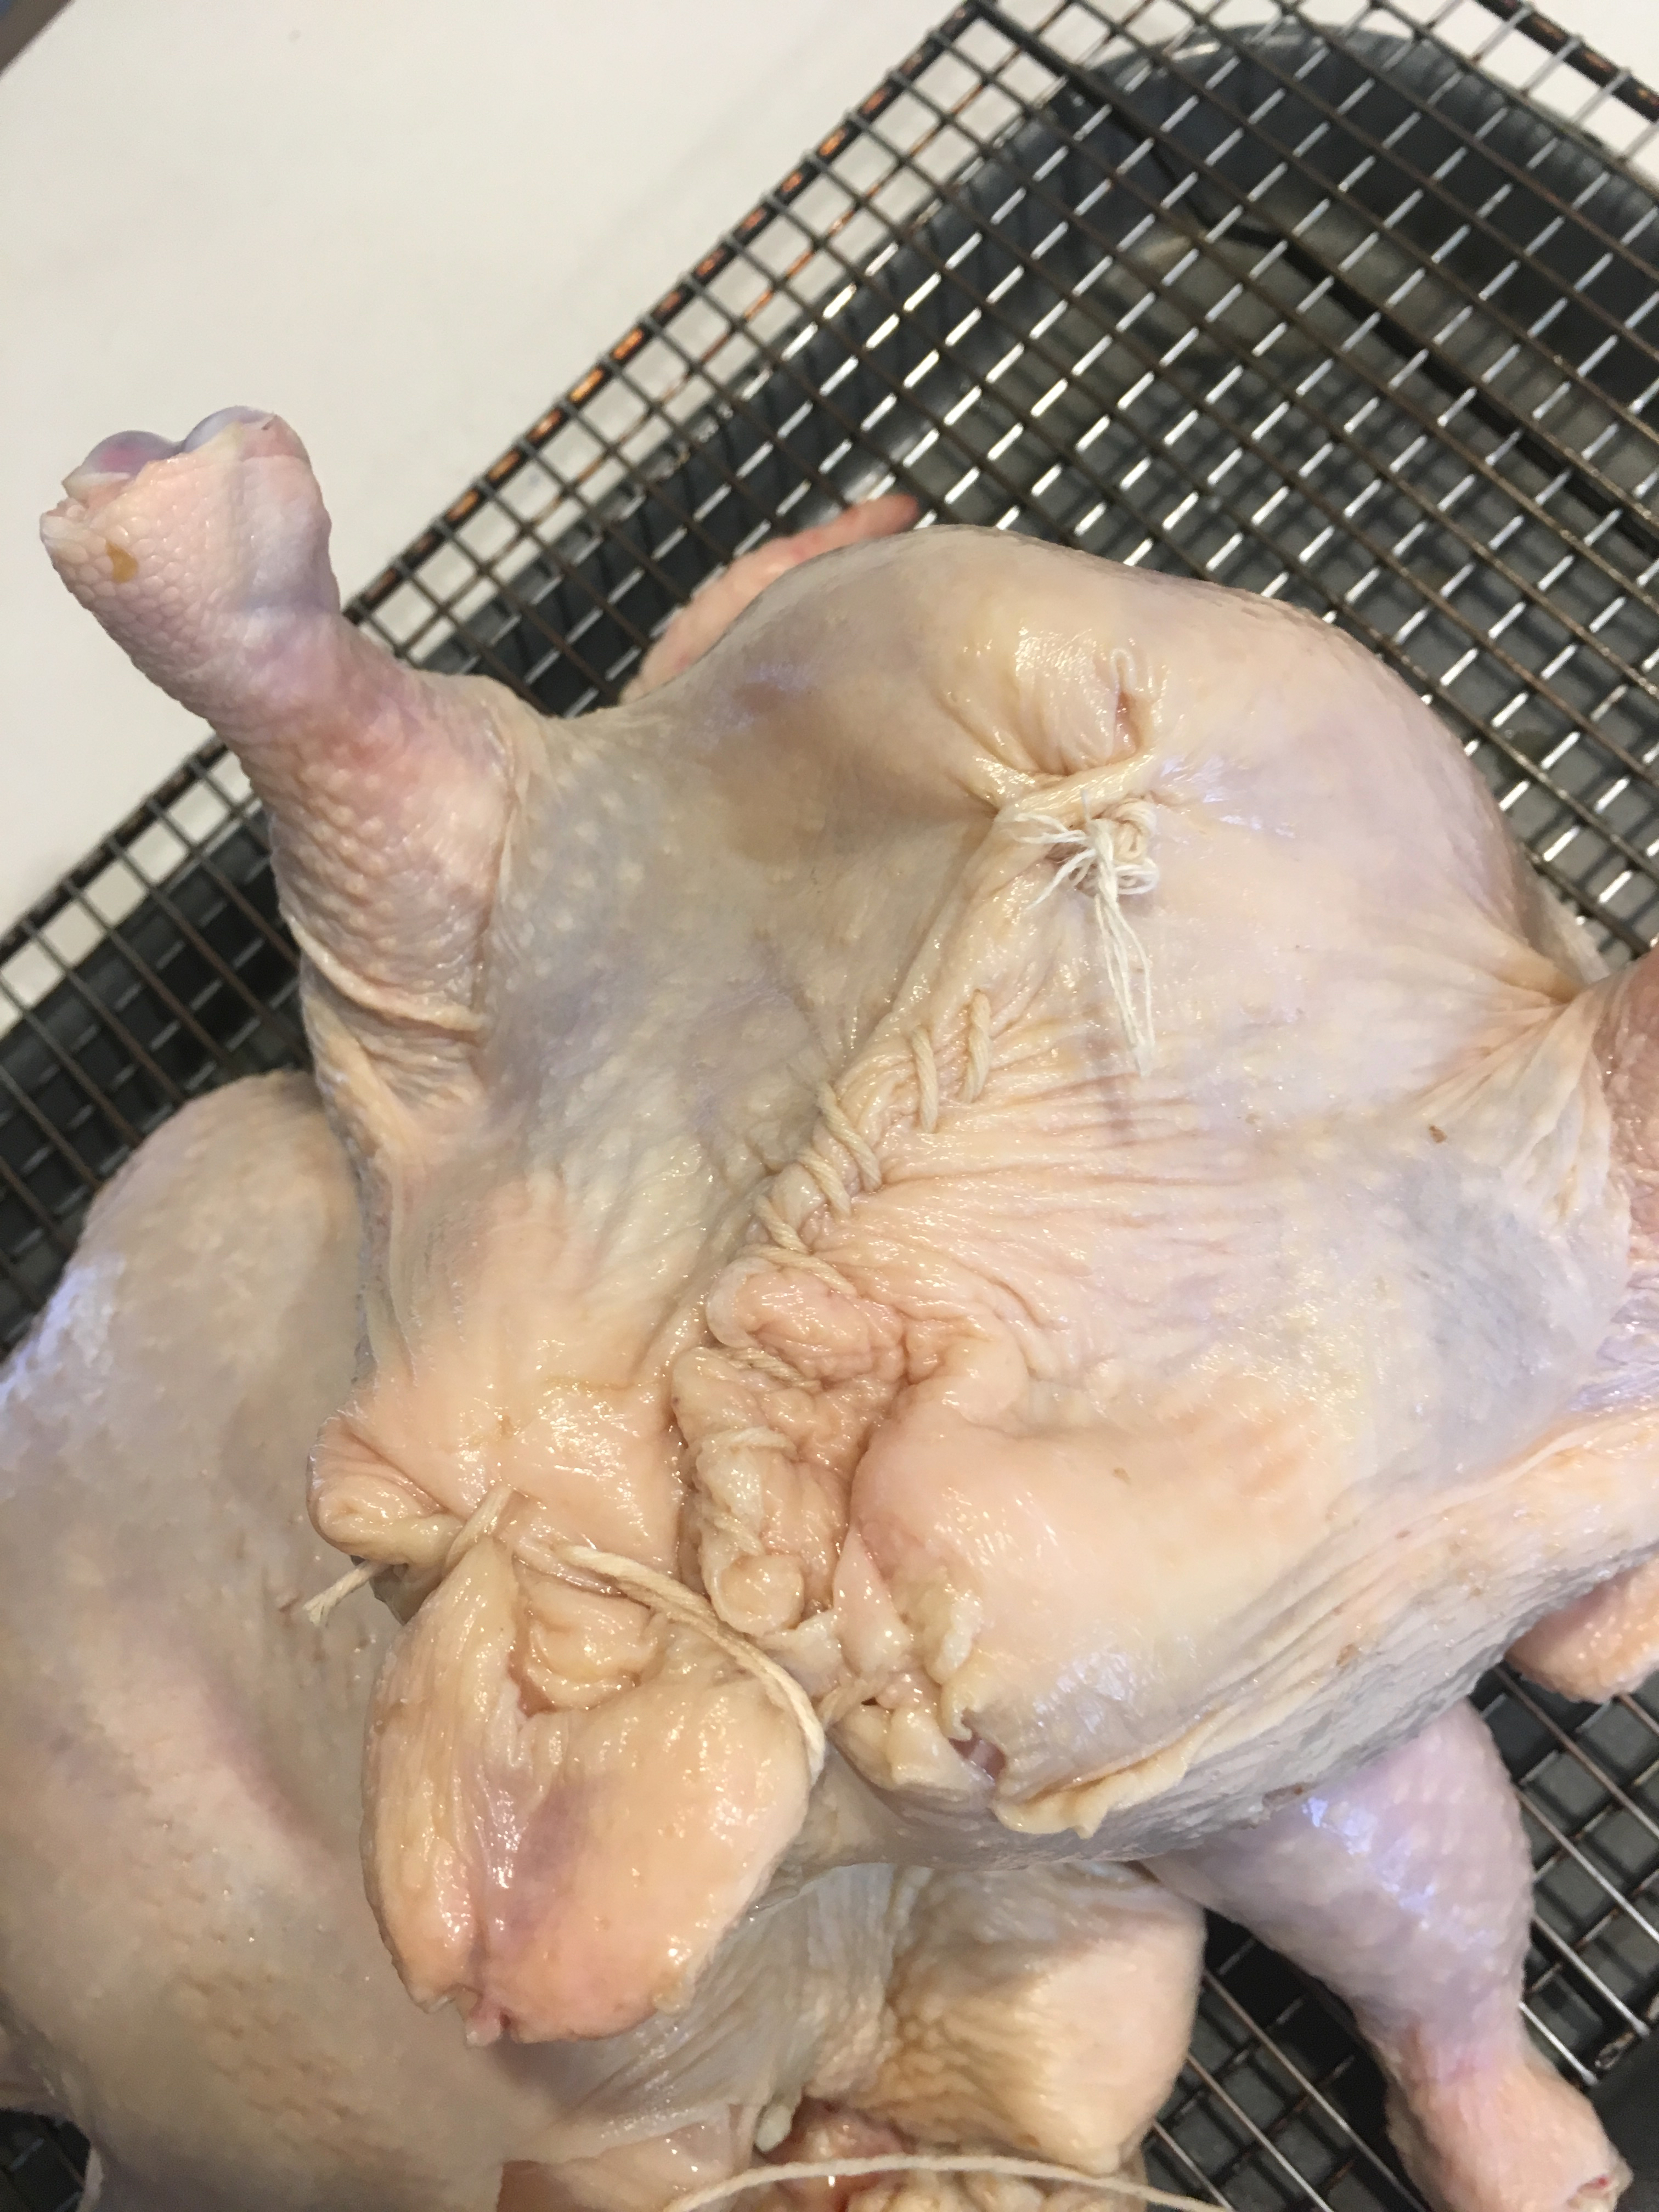
\includegraphics[width=0.25\textwidth]{\imageDir/\fileName/IMG_3217.jpg} &
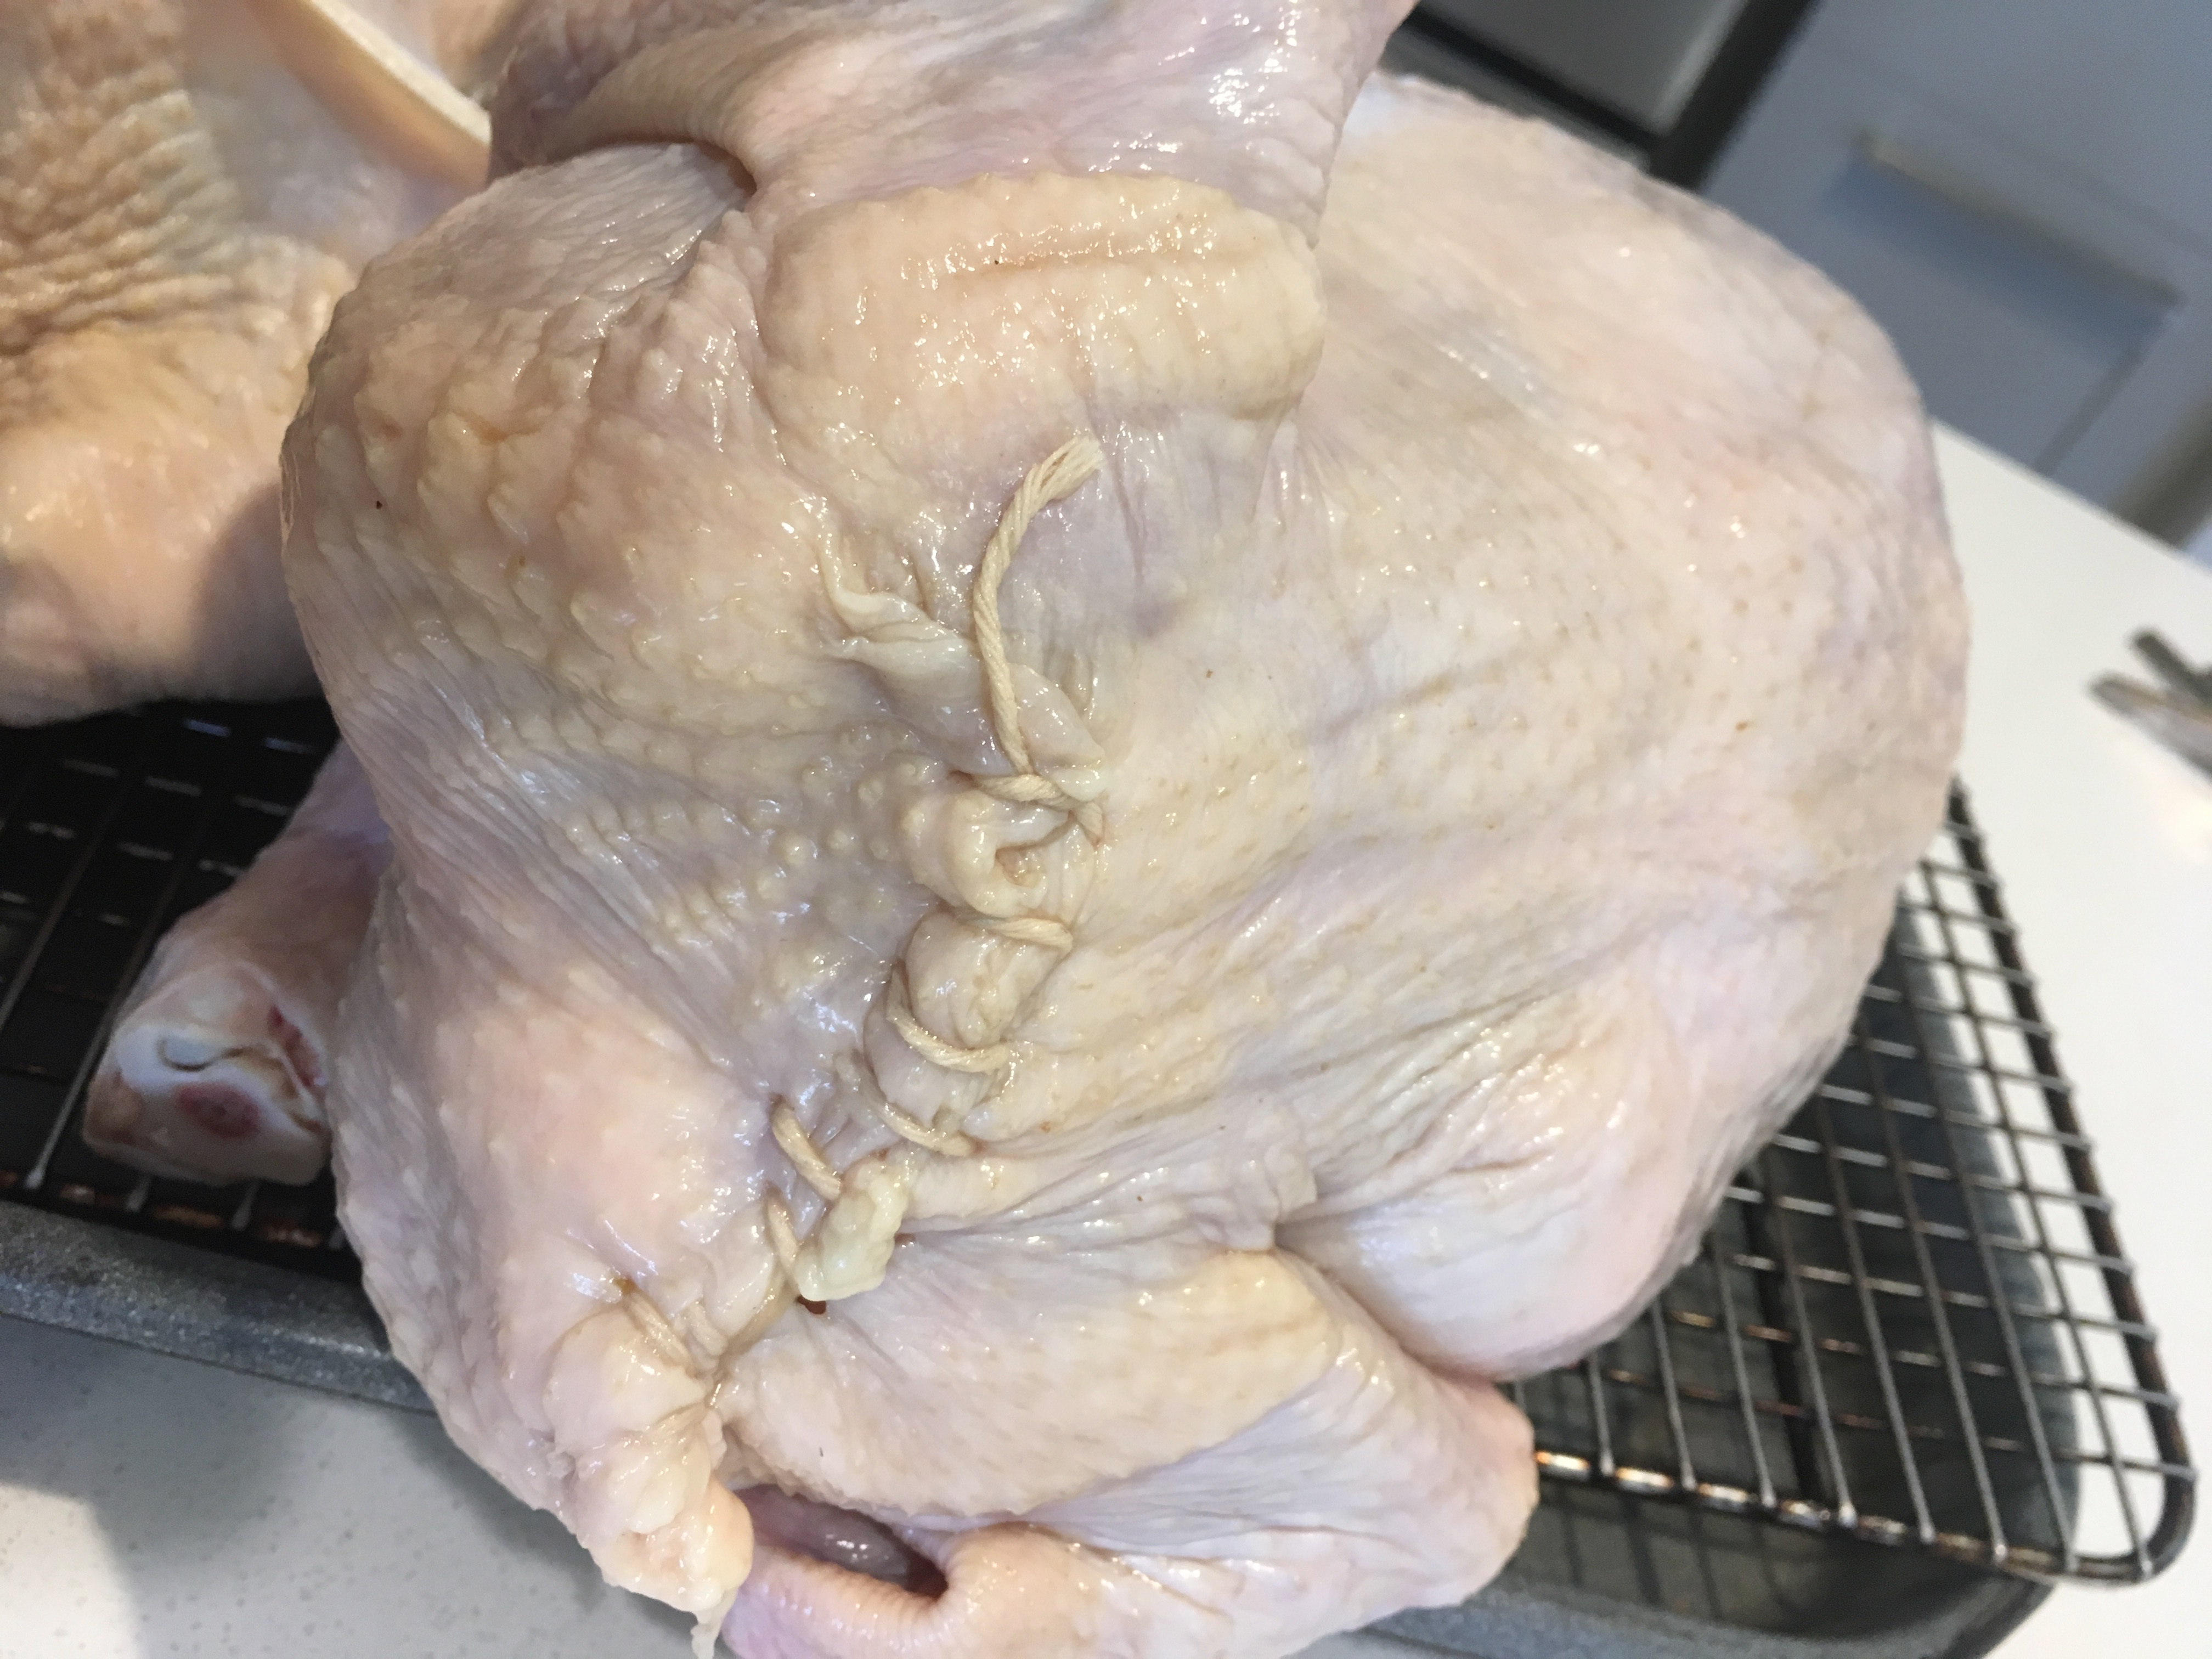
\includegraphics[width=0.25\textwidth]{\imageDir/\fileName/IMG_3218.jpg} &
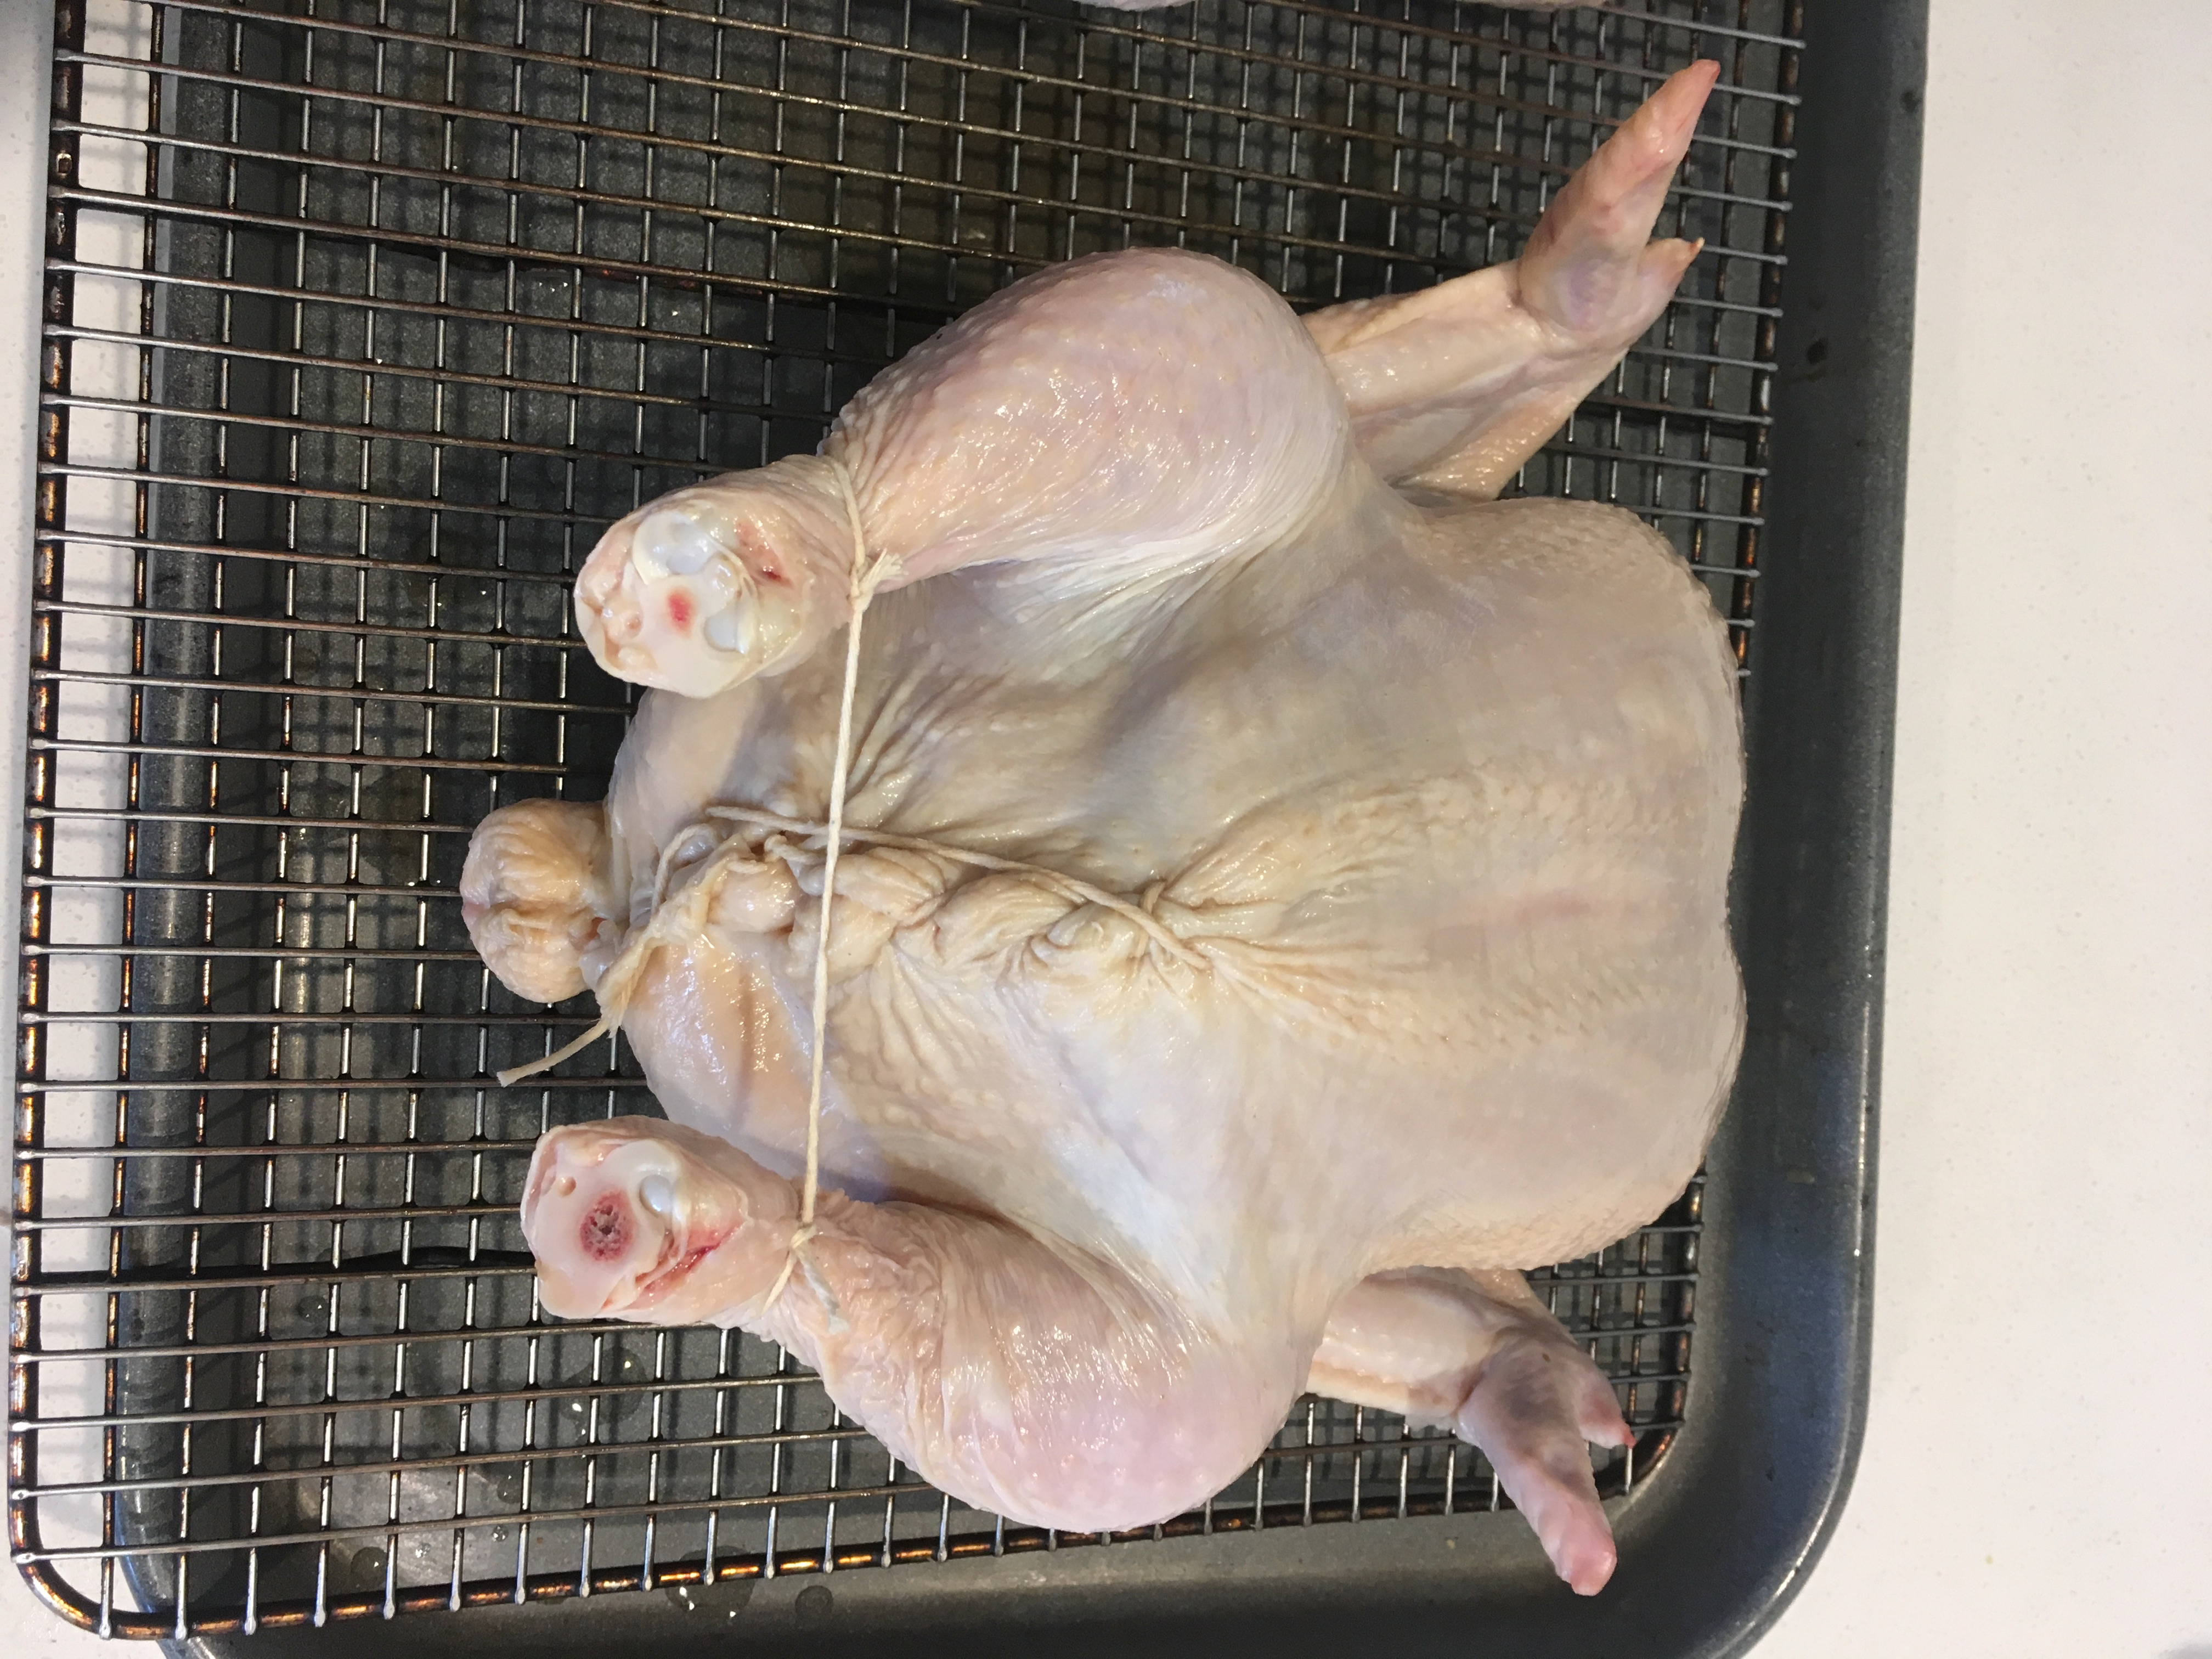
\includegraphics[width=0.25\textwidth]{\imageDir/\fileName/IMG_3219.jpg} \\
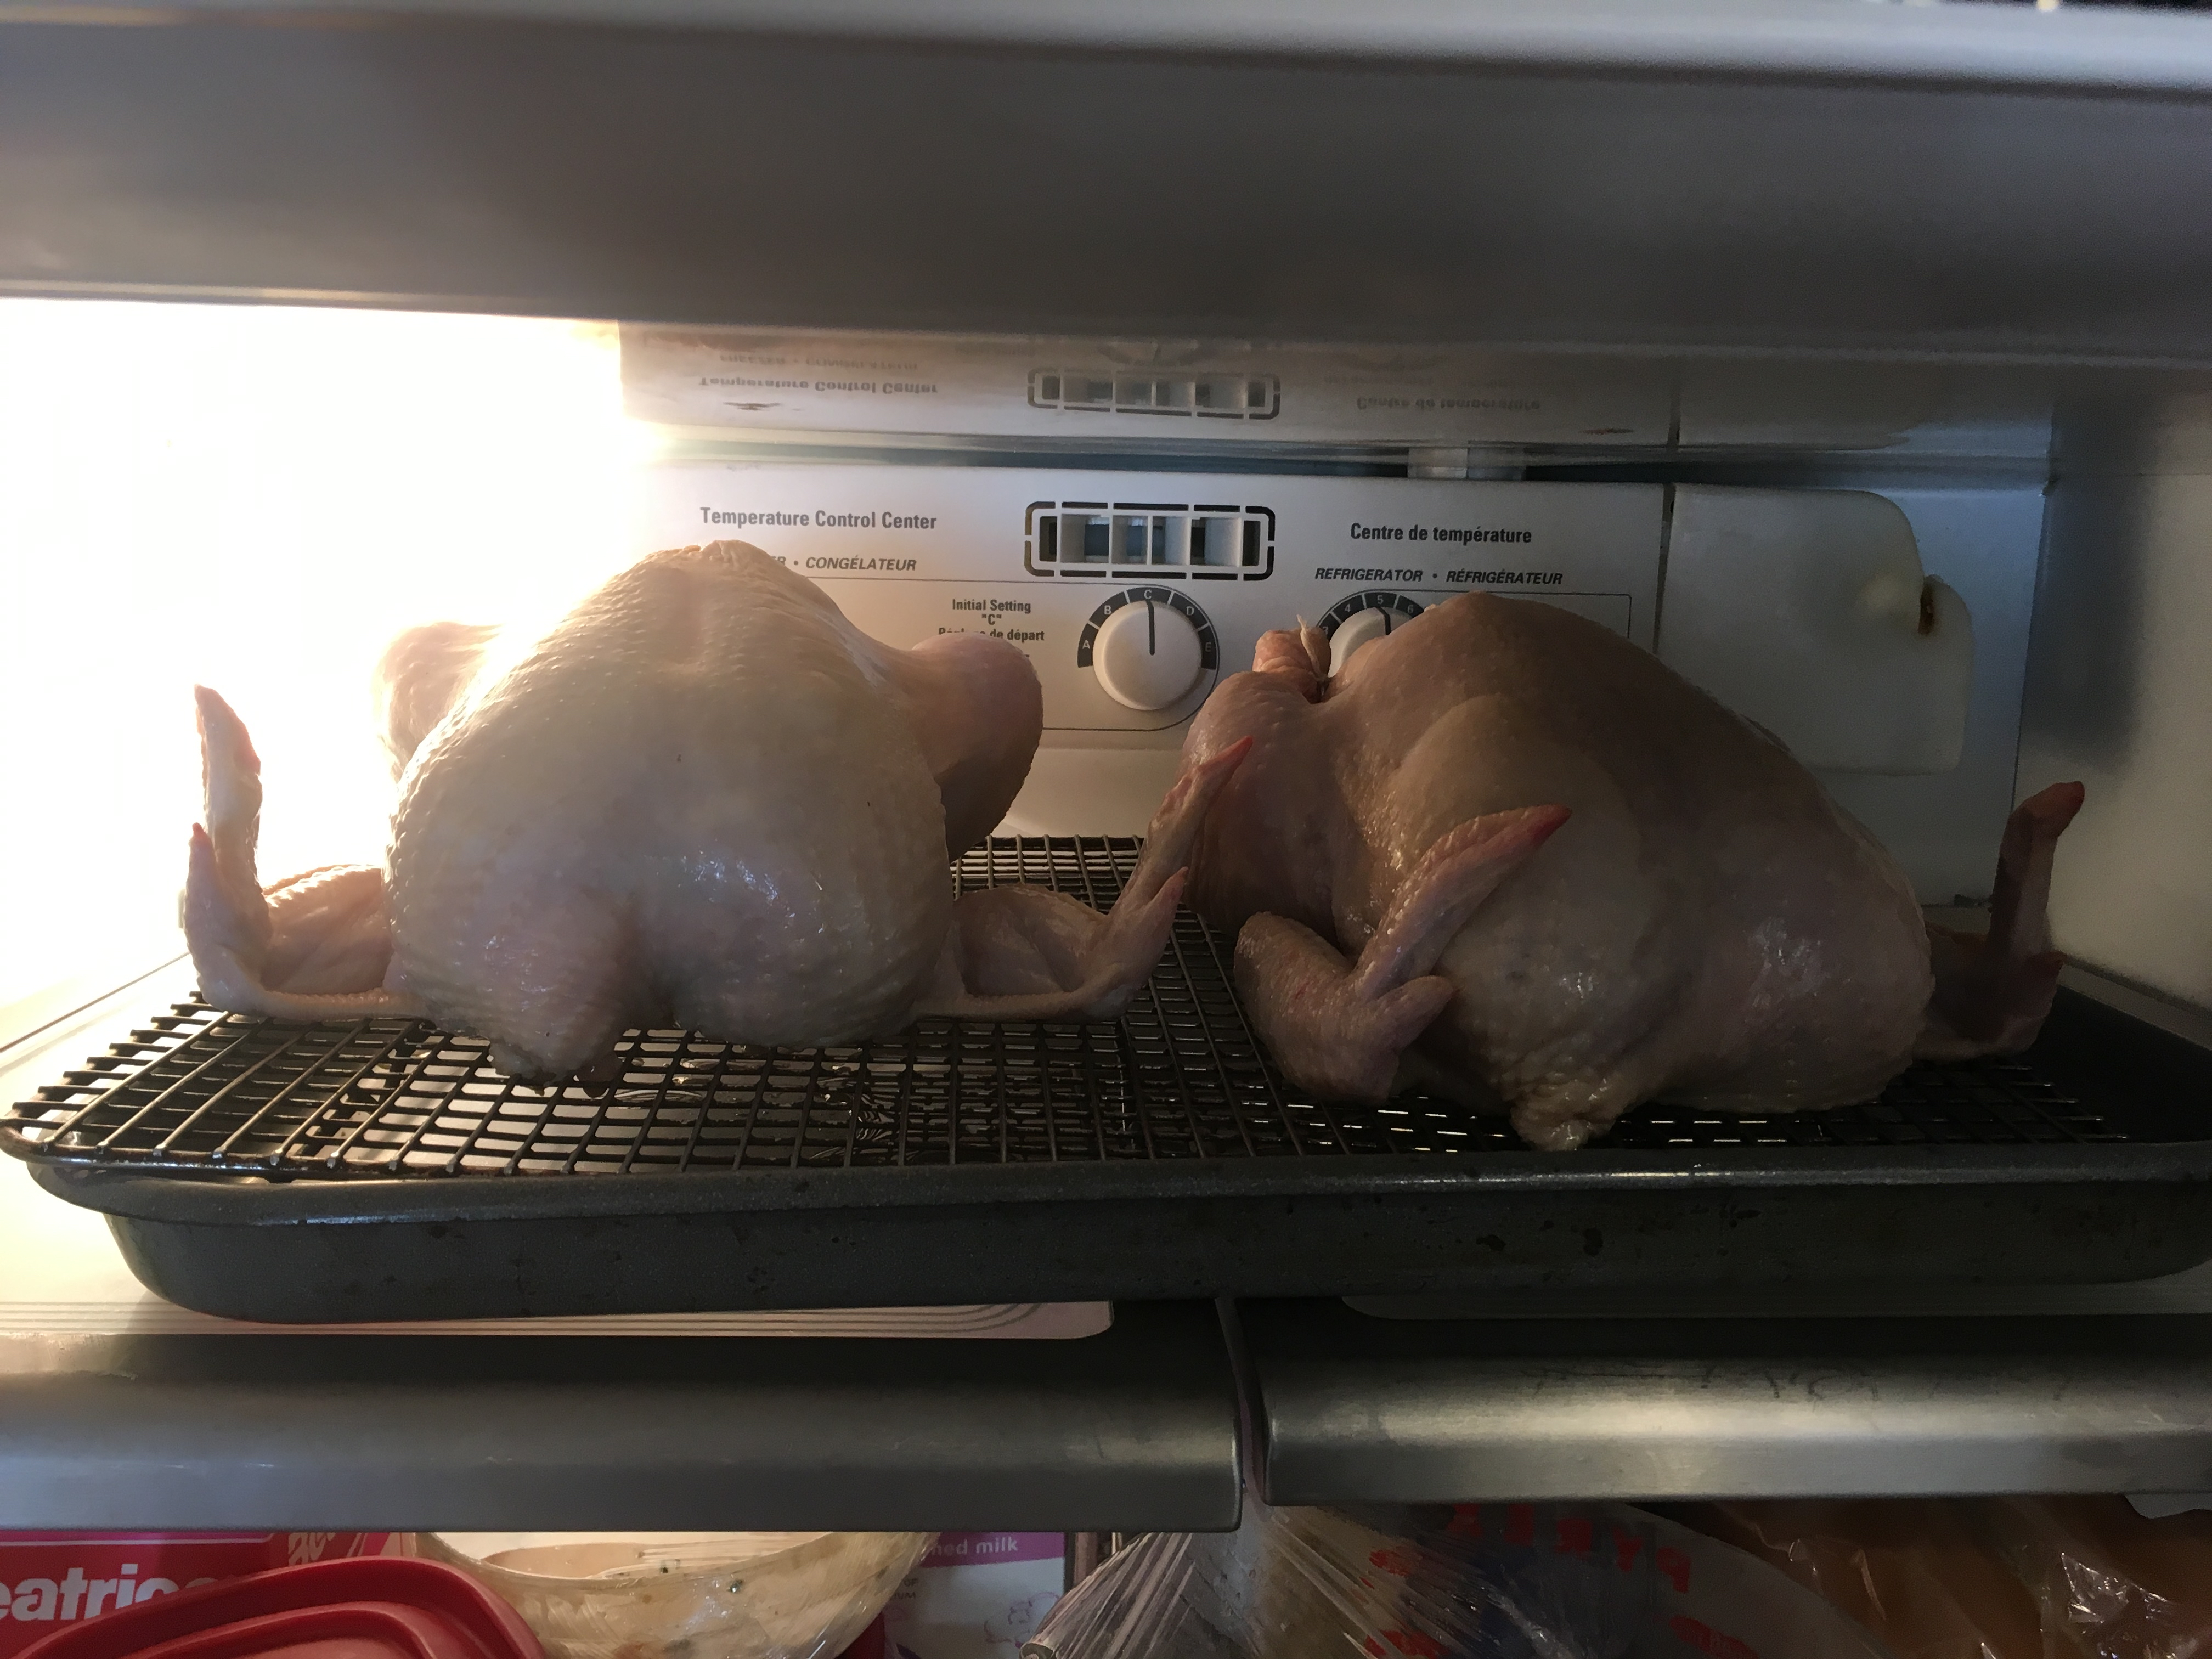
\includegraphics[width=0.25\textwidth]{\imageDir/\fileName/IMG_3220.jpg} &
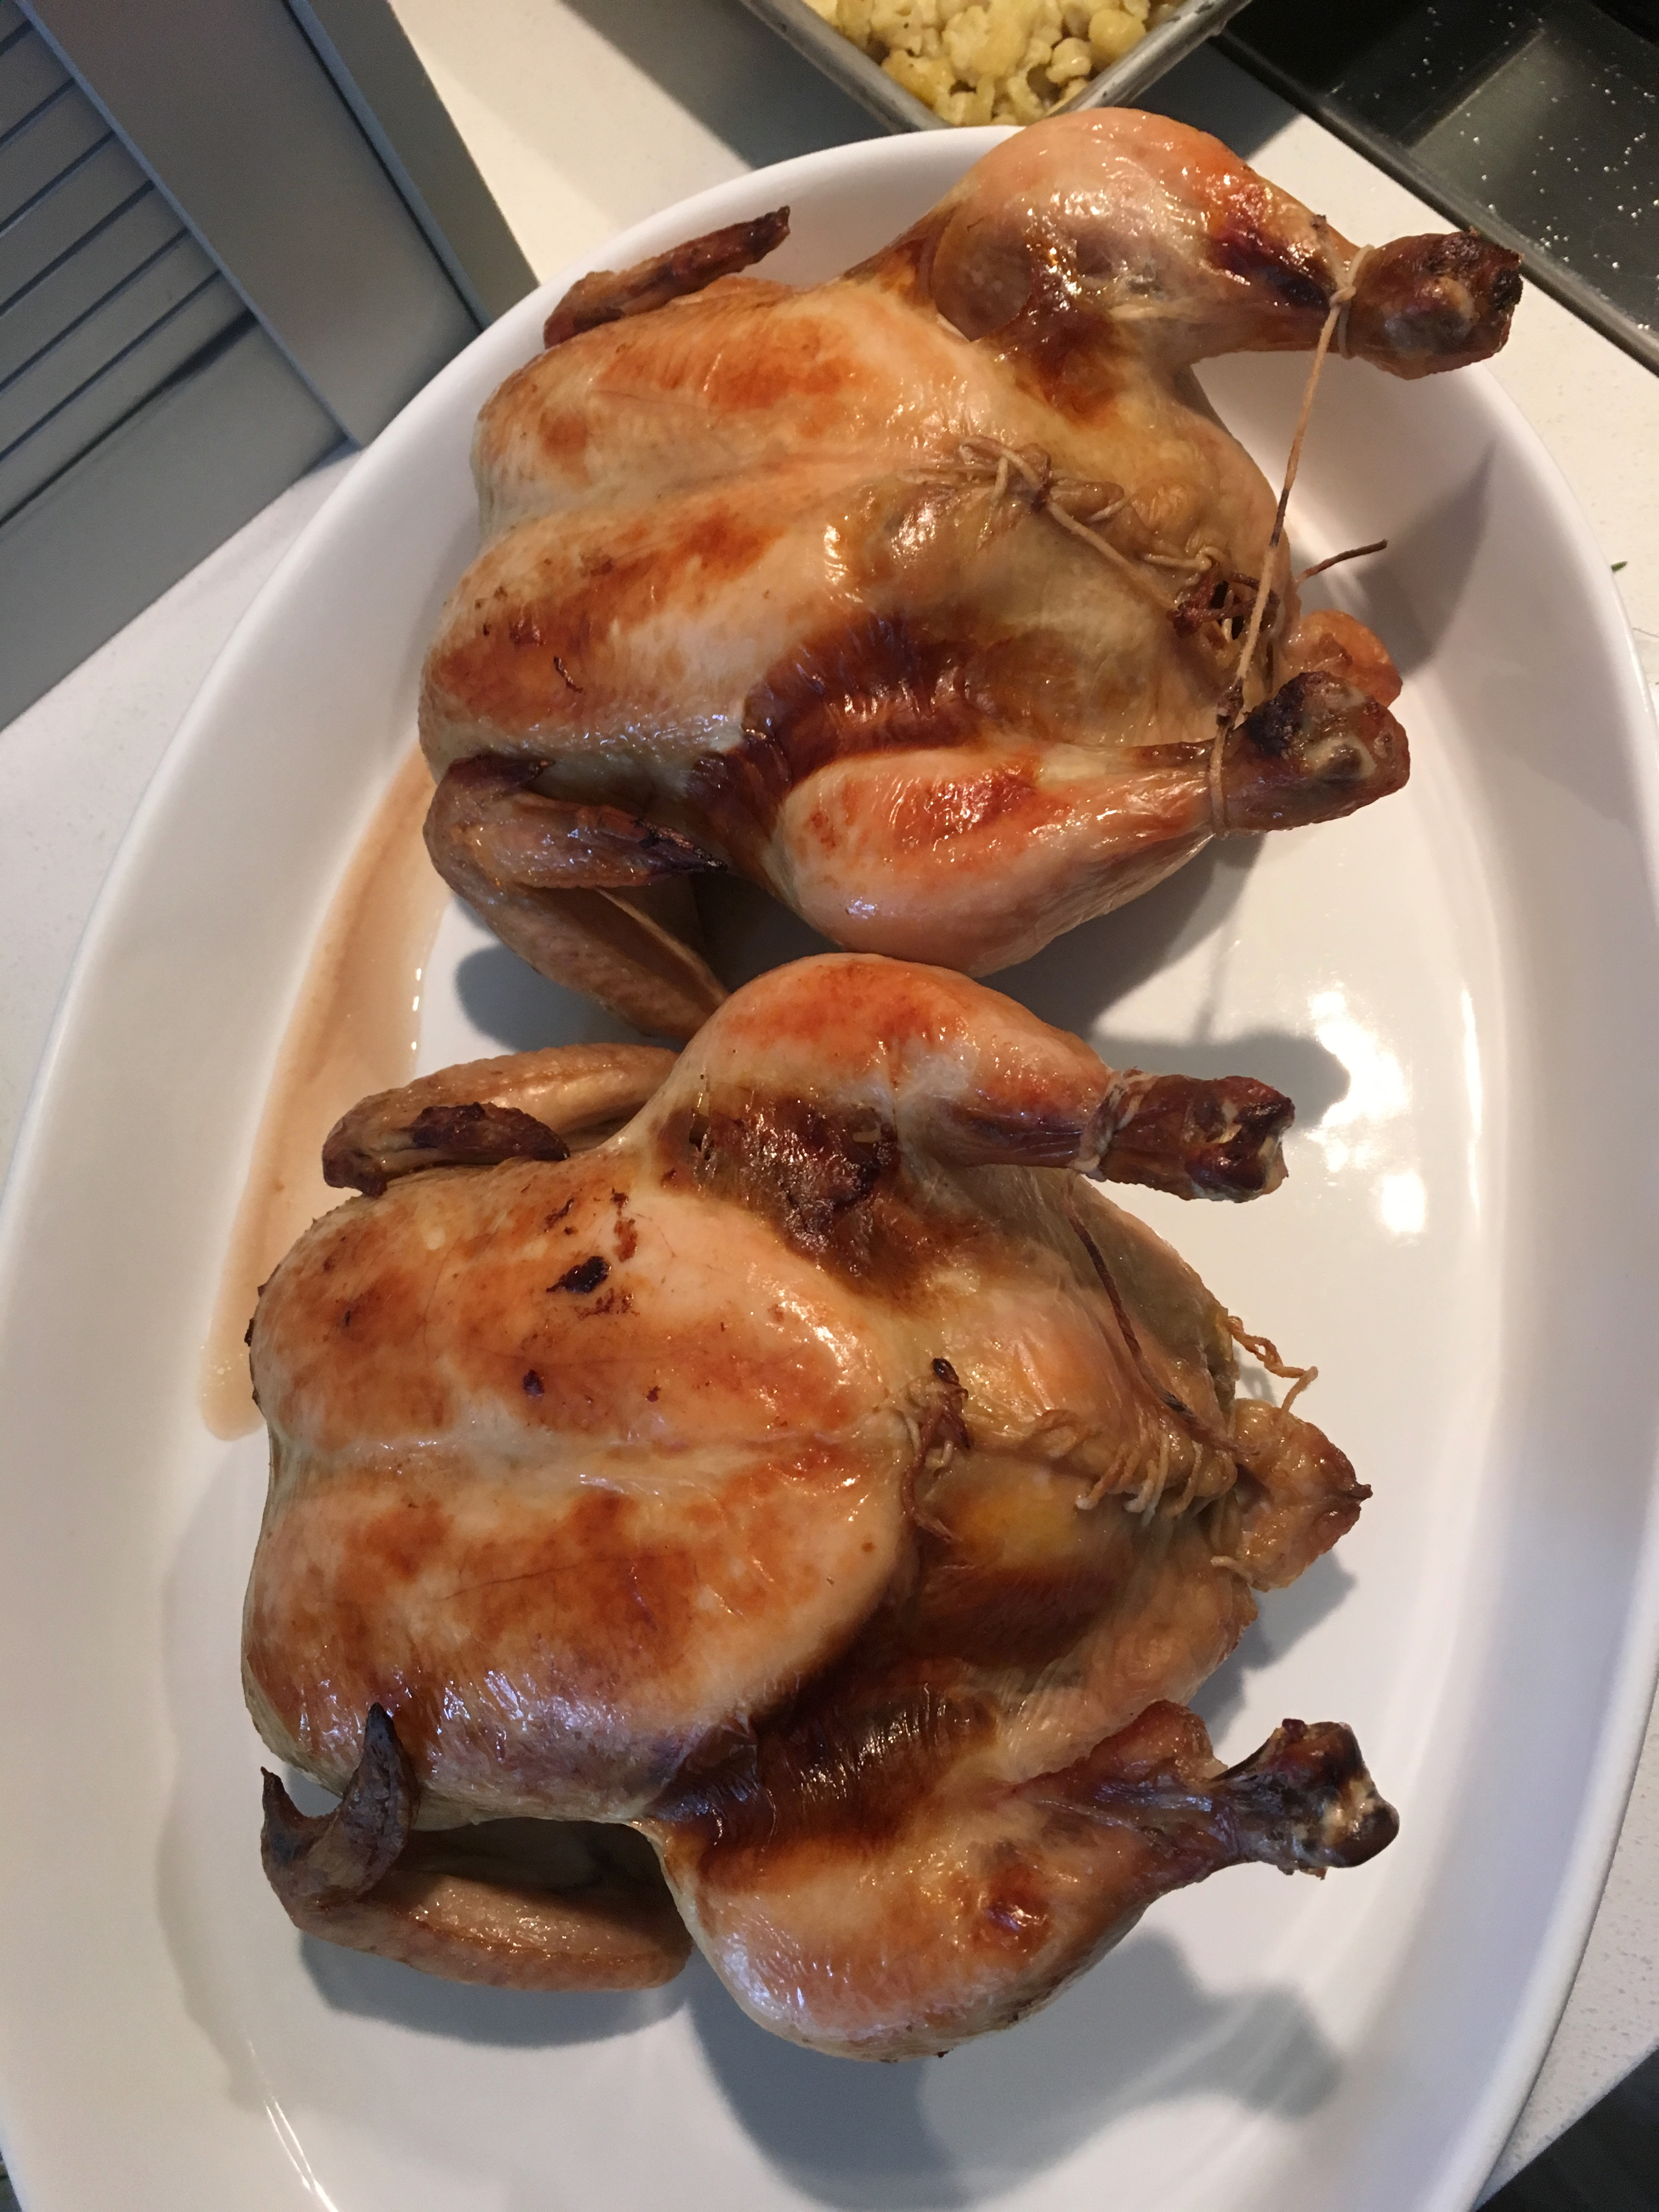
\includegraphics[width=0.25\textwidth]{\imageDir/\fileName/IMG_3228.jpg} \\
\end{tabular}
\end{table}


\end{document}
